\documentclass{article}
\usepackage[utf8]{inputenc}
\usepackage[round]{natbib}
\usepackage[table,xcdraw,dvipsnames]{xcolor}
\usepackage{graphicx}
\usepackage{caption}
\usepackage{authblk}
\usepackage{textgreek}
\usepackage{rotating}
\usepackage{breakcites}

\newcommand{\amw}[1]{{\textcolor{OliveGreen}{AW: #1}}} % %edit
\newcommand{\pjw}[1]{{\textcolor{blue}{PW: #1}}} % %edit
\newcommand{\dfw}[1]{{\textcolor{OrangeRed}{DW: #1}}} % %edit


\title{Testing character evolution models in phylogenetic paleobiology: a case study with Cambrian echinoderms}
%Pete to others: I shifted it to "evolution" models because we get at a little more than clocks here, or at least more than most paleontologists would associate with clocks

%Davey- For a working title, how about something like, "Testing character-based clock models in phylogenetic paleobiology: a case study with Cambrian echinoderms?" Feel free to change it up now and/or as we move along!

% Davey--Should we change the title? Or is this still appropriate?

\author[1]{April M. Wright}
\author[2]{Peter J. Wagner}
\author[3,4]{David F. Wright}

%Davey- I assume this is the correct order (but feel free to change if I'm wrong!) Check the institutional affiliations to make sure I got them correct!
\affil[1]{Department of Biological Sciences, Southeastern Louisiana University, 2400 N Oak St., Hammond, LA, 70402 USA}
\affil[2]{Department of Earth and Atmospheric Sciences, and School of Biological Sciences, University of Nebraska Lincoln, Lincoln, NE 68588-0340, USA.}
\affil[3]{Department of Paleobiology, National Museum of Natural History, Smithsonian Institution, Washington DC, USA}
\affil[4]{Division of Paleontology, American Museum of Natural History, New York, USA}
\date{December 2020}

\begin{document}

\maketitle

\section{Abstract}

Macroevolutionary modeling has historically been treated as a two-step process, involving the inference of a phylogenetic tree, and then fitting of a macroevolutionary model using that tree.
Newer models, such as the fossilized birth-death model, blend the two steps.
These methods make more complete use of fossils than the previous generation of Bayesian phylogenetic models.
They also involve many more parameters than prior models, including parameters about which empiricists may have little intuition.
In this paper, we set forth a framework for fitting complex, hierarchical models.
We ultimately fit and use a joint tree and diversification model to estimate a dated phylogeny of the Cincta (Echinodermata), a morphologically distinct group of Cambrian echinoderms that lack the five-fold radial symmetry characteristic of extant members of the phylum.
Although the phylogeny of cinctans remains poorly supported in places, we show how models of character change and diversification can contribute to understanding patterns of phylogenetic relatedness and testing macroevolutionary hypotheses. 

\section{Introduction}

Historically, drawing macroevolutionary inferences from phylogenetic trees has been a two-step process \citep{Harvey1991}.
First, a researcher would estimate a phylogenetic tree from a matrix of phylogenetic characters (typically morphological characters or molecular sequence characters).
Then, they would use that tree (or a set of trees, such as a posterior sample) to fit a macroevolutionary model.
Over the past decade, models that blend macroevolutionary inference with phylogenetic inference have become increasing common.
For example, the fossilized birth-death process is used to estimate dated phylognetic trees \citep{Stadler2011, Heath2014}.
This process is usually implemented as a Bayesian hierarchical model, in which one model describes the process of character change for phylogenetic characters, one describes the distribution of evolutionary rates over the tree, and one describes the process of speciation, extinction, and sampling that lead to the observed tree (see Warnock and Wright in this issue for a more complete discussion of this).
In this manuscript, we describe an approach to fitting complex hierarchical models using a focal dataset of cinctan echinoderms.

We can divide macroevolutionary hypotheses into two non-mutually exclusive groups: those making predictions about origination and extinction dynamics, and those making predictions about rates and modes of trait evolution. 
The latter group includes hypotheses about shifts in rates of anatomical change and hypotheses about driven trends in which particular character states become more (or less) common over time.  
Hypotheses predicting such patterns come both from macroecological theory and from evolutionary‑developmental theory, and thus span a range of basic issues including developmental, ecological, and physical constraints, and selection  \citep{valentine1969patterns, valentine1980determinants}
Research programs dedicated to assessing shifts in rates and modes of anatomical evolution have been staple of quantitative paleobiology since the early 1990’s. 
Accordingly, anatomical character evolution models that describe the predictions of these different macroevolutionary hypotheses have important theoretical implications for these endeavors. 

Phylogeneticists have long been interested in the same sorts of character evolution models, albeit for very different reasons.  
Hypotheses of phylogenetic relationships make exact predictions about character state evolution among taxa given observed data and models of character change (e.g., \cite{Kimura1980, Felsenstein1981, Hasegawa1985, Tavare1986}).  
The most common phylogenetic model for morphology makes the assumption of time-invariant models with no biases in the rate of character acquisition and loss \citep{Lewis2001}.
The expectations of character evolution, of associations of characters with one another, and disparities between taxa are very different when rates of acquisition and loss vary among characters and with time.
This is particularly true when we include divergence times as part of phylogenetic hypotheses \citep{Huelsenbeck2000a, Sanderson2002, Drummond2006}: but it is still true if we worry only about general cladistic relationships (i.e., which taxa are most closely related to each other; see \cite{Felsenstein1981, Nylander2004, Wright2016}).  
In other words, many of the conceptual mice that paleobiologists seek to capture are the conceptual mouse-traps that systematists seek to use to capture phylogenies.  

Many readers’ first instincts will be that this presents paleobiological phylogeneticists with a quandary: which comes first, the character evolution models or the phylogenetic inference?  
%This is particularly true because one of the reasons why paleobiologists often choose particular clades for phylogenetic analyses is that the taxon represents an appropriate system for assessing alternative hypotheses about macroevolutionary dynamics, including those positing different types of character evolution models.  
%For example, our alternate ideas for explaining early bursts of disparity (e.g., declining rates of change vs. limited character space; see Foote 1997) or active trends (e.g., driven trends [= biased state change] vs. species selection or phylogenetic effects; see \cite{raup1974, stanley1975; mcshea1994}) correspond to different models of character evolution in phylogenetic analyses. 
%Moreover, such hypotheses apply to many or all of the characters available to paleontologists for study, there usually no recourse to “independent” character data for phylogenetic analysis such as was commonly prescribed for tree‑based macroevolutionary studies (e.g., Harvey and Pagel 1991).
%Another way to look at this is the Catch-22 that might arise if we were to submit a paper about phylogenetic relationships to a journal such as Journal of Paleontology and a paper about a macroevolutionary issue such as shifts in rates of anatomical change to a journal such as Paleobiology with both papers using the same data set.  
%For the phylogeny paper, we (should!) need to convince reviewers and editors that the models of character change are sufficiently complex that we can trust the resulting phylogeny. For the rate-shift paper, we (should!) need to convince reviewers and editors that the null hypotheses, i.e., continuous rates of change over time (i.e., strict clocks) are inadequate before rejecting them in favor of the more complex idea that rates changed over time.  In other words, our burdens of proof run in opposite directions even though we actually are discussing the same sets of evolutionary parameters and simply putting more emphasis on one set or another.  
Part of the dilemma here stems from a historical view that we should treat phylogenetic analysis and macroevolutionary analysis as two separate endeavors (e.g., \cite{Harvey1991}).  
When we estimate a phylogenetic tree, we typically need to make simplifying assumptions about the evolution of our phylogenetic characters for tractability of the analysis.
For our comparative methods, we are often using a smaller subset of the data to explore more complex models, possibly even seeking to falsify those same simplifying assumptions.
Here, we advocate a very different approach that stems from hierarchical Bayesian phylogenetic approaches.  
That is, we should not view phylogenetic analysis and macroevolutionary analysis as two independent projects, but instead as two parts of the same endeavor of unravelling the evolutionary history of fossil taxa.  
These evolutionary histories include when clades and lineages diverged, the consistency of character change rates, biases in state acquisition, the process of diversification that lead to the observed tree, and (of course) exactly how taxa were related to each other.  
Along the same lines, we have to accept and even embrace the fact that there will always be some degree of uncertainty in all of these things.  
These uncertainties are not reason to abandon the endeavor as hopeless; on the contrary, it will mean that those conclusions that we can reach do not assume that specific historical details are true.  

In this work, we will provide an example of the approach that we are advocating using a series of analyses of the Cincta, an extinct clade of `carpoid' echinoderms from the middle Cambrian. 
We will detail how paleobiologists can adapt different clock models and character state evolution models initially devised to accommodate uncertainties in molecular evolution to represent and model macroevolutionary hypotheses.  
In doing so, we will also outline protocol that paleontologists can replicate to conduct analogous analyses on other clades.  
We will emphasize how the combination of Markov Chain Monte Carlo analyses and stepping‑stone tests allow us to marginalize specific details of character evolution models and phylogenetic relationships in order to generate the best joint summary of a clade’s evolutionary history.  
Because there are innumerable possible models that one might consider, we will draw attention to existing methods with which paleontologists might already be familiar that should be useful for suggesting particular models as worthy of consideration.  
Finally, we will briefly outline other theoretical and methodological areas that remain for paleobiologists and systematists to resolve and unite in the future. 

\section{Taxonomic Background and Data}
\subsection{Cincta: an enigmatic clade of Cambrian echinoderms}

Echinoderms are a diverse phylum of marine animals represented today by more than 7,000 living species \citep{brusca2003} distributed among five extant classes, including sea stars, brittle stars, echinoids, sea cucumbers, and crinoids. However, the spectacular diversity of extant echinoderms, measured by both species richness and anatomical variety, represents a paltry fraction of their prodigious evolutionary history recorded in the fossil record. Because echinoderms possess a mineralized endoskeleton made of high-magnesium calcite (calcium carbonate) and occur in virtually all habitats across the spectrum of marine depositional environments, the echinoderm fossil record is spectacularly complete and reveals approximately 30 clades distributed among 21 taxonomic classes spanning the entire Phanerozoic Eon \citep{SprinkleKier1987, Sumrall1997, SumrallWaters2012, ZamoraRahman2014, WrightEtAl2017, SheffieldSumrall2019}. Unlike familiar echinoderms inhabiting modern oceans, such as sea stars and sea urchins (echinoids), Cambrian lineages comprise an unfamiliar, taxonomically and morphologically diverse assemblage of predominately stem-group taxa exhibiting a diversity of body plans, life modes, and ecological traits unseen in extant lineages \citep{Sprinkle1973, ZamoraEtAl2013, ZamoraRahman2014}.

Perhaps no group of early echinoderms has received greater attention and controversy than the `carpoids’ \citep{RahmanMakingSenseofCarpoids2009}. Sometimes called homalozoans or calcichordates in the literature, carpoids comprise a heterogenous assemblage of extinct echinoderms including ctenocystoids, cinctans (Homostelea), solutes (Homoiostelea), and stylophorans. Although carpoids possess unique skeletal features that unambiguously identify their echinoderm affinities \citep{DavidEtAl2000, Bottjer2006, RahmanMakingSenseofCarpoids2009, ZamoraEtAl2020}, they lack other traits considered synapomorphies of crown-group echinoderms. For example, all extant echinoderms exhibit pentaradial symmetry in adults and possess a water vascular system, unique to the phylum, used for locomotion, respiration, and excretion \citep{Nichols1972}.  In contrast, ‘carpoid’ taxa exhibit bilateral to asymmetrical forms, and it’s debated whether some possessed a water vascular system \citep{Smith2005, LefebvreEtAl2019}. Although the phylogenetic position of carpoids have long been contentiously debated (see \citealp{RahmanMakingSenseofCarpoids2009} and \citealp{Rahman2009b}, and articles cited therein), only recently have computer-based phylogenetic analyses played a major role in evaluating alternative hypotheses \citep{Sumrall1997, SmithAndZamora2013, ZamoraRahman2014}, and only one previous study tested phylogenetic hypotheses using stratigraphic data \citep{Rahman2009b}. Crucially, the character matrices constructed for these analyses have greatly benefited from recent improvements to identifying homologous characters across morphologically disparate early echinoderm lineages, often arising from new fossil discoveries (e.g., \citealp{ZamoraEtAl2012, SmithAndZamora2013}). Taxonomic controversy remains \citep{DavidEtAl2000}, though both recent computational phylogenetic analyses and stratigraphic congruence metrics support the hypothesis that carpoids comprise a paraphyletic assemblage of stem-group echinoderms \citep{Rahman2009b, SmithAndZamora2013, ZamoraRahman2014}. If this view is correct, then carpoids help document the radical transition in echinoderm evolution from an ancestral, bilaterian body plan to the pentaradial symmetry characteristic of crown-group forms that have dominated marine ecosystems since the close of the Cambrian. Regardless of their specific branching relationships in the echinoderm tree of life, it is nevertheless clear that understanding the distribution of character combinations and patterns of trait evolution in these enigmatic, pre-radial echinoderm lineages are critical to deciphering the early evolution of the phylum.

Cinctans are a significant group of non-radiate, carpoid echinoderms temporally restricted to the middle Cambrian (Miaolingian 509—497 Ma, with ocurrences of Cinctans from 506.6 - 297 Ma) and paleogeographically restricted to western Gondwana, Avalonia, and Siberia. Cinctans are generally small (i.e., several 1 to 10 mm in length), flattened, symmetrical to irregularly shaped fossils resembling a tennis racquet or badly formed pancake, generally interpreted as an adaptation to an epibenthic, suspension feeding lifestyle \citep{Rahman2009a, RahmanEtAl2015}.  Like all echinoderms, cinctans have a complex, multi-element, calcitic endoskeleton, which makes them particularly amenable for coding discrete, phylogenetic characters in fossil taxa \citep{SmithZamora2009}. The main body, called the theca, is surrounded by a series of rigid, stout, marginal plates (called the cinctus), which surrounds a central body of smaller, tessellated integument plates on both dorsal and ventral sides. The mouth is a circular opening located at the end of a narrow food groove (or pair of grooves) on the right anterior side of the theca. A posterior appendage, called the stele, forms a rigid structure extending from the cinctus, commonly subequal in length to the theca (Figure 1).

Despite their diminutive size, geological antiquity, and narrow paleogeographic and stratigraphic ranges, the significance of cinctans to understanding early echinoderm evolution, as well as their evolutionary implications surrounding ancestral character states in ancient deuterostomes \citep{SmithSwalla2009}, has led to a substantial amount of interest to decipher their paleobiology. Recent advances in cinctan paleobiology include efforts to better understand patterns of taxonomic diversity \citep{ZamoraAlvaro2010}, ontogeny and development \citep{Smith2005,ZamoraRahmanSmith2013}, life mode and feeding ecology \citep{Rahman2009b, RahmanEtAl2015,ZamoraRahman2015}, convergence and adaptive evolution \citep{ZamoraSmith2008} and phylogenetic relationships \citep{Freidrich1993, Sdzuy1993, SmithZamora2009, ZamoraRahmanSmith2013}. In this study, we combine morphological data with fossil age information to re-evaluate phylogenetic relationships and evolutionary dynamics among cinctan lineages using hierarchical Bayesian phylogenetic models and provide a phylogenetic template for future systematic and macroevolutionary studies.
\begin{figure*}
  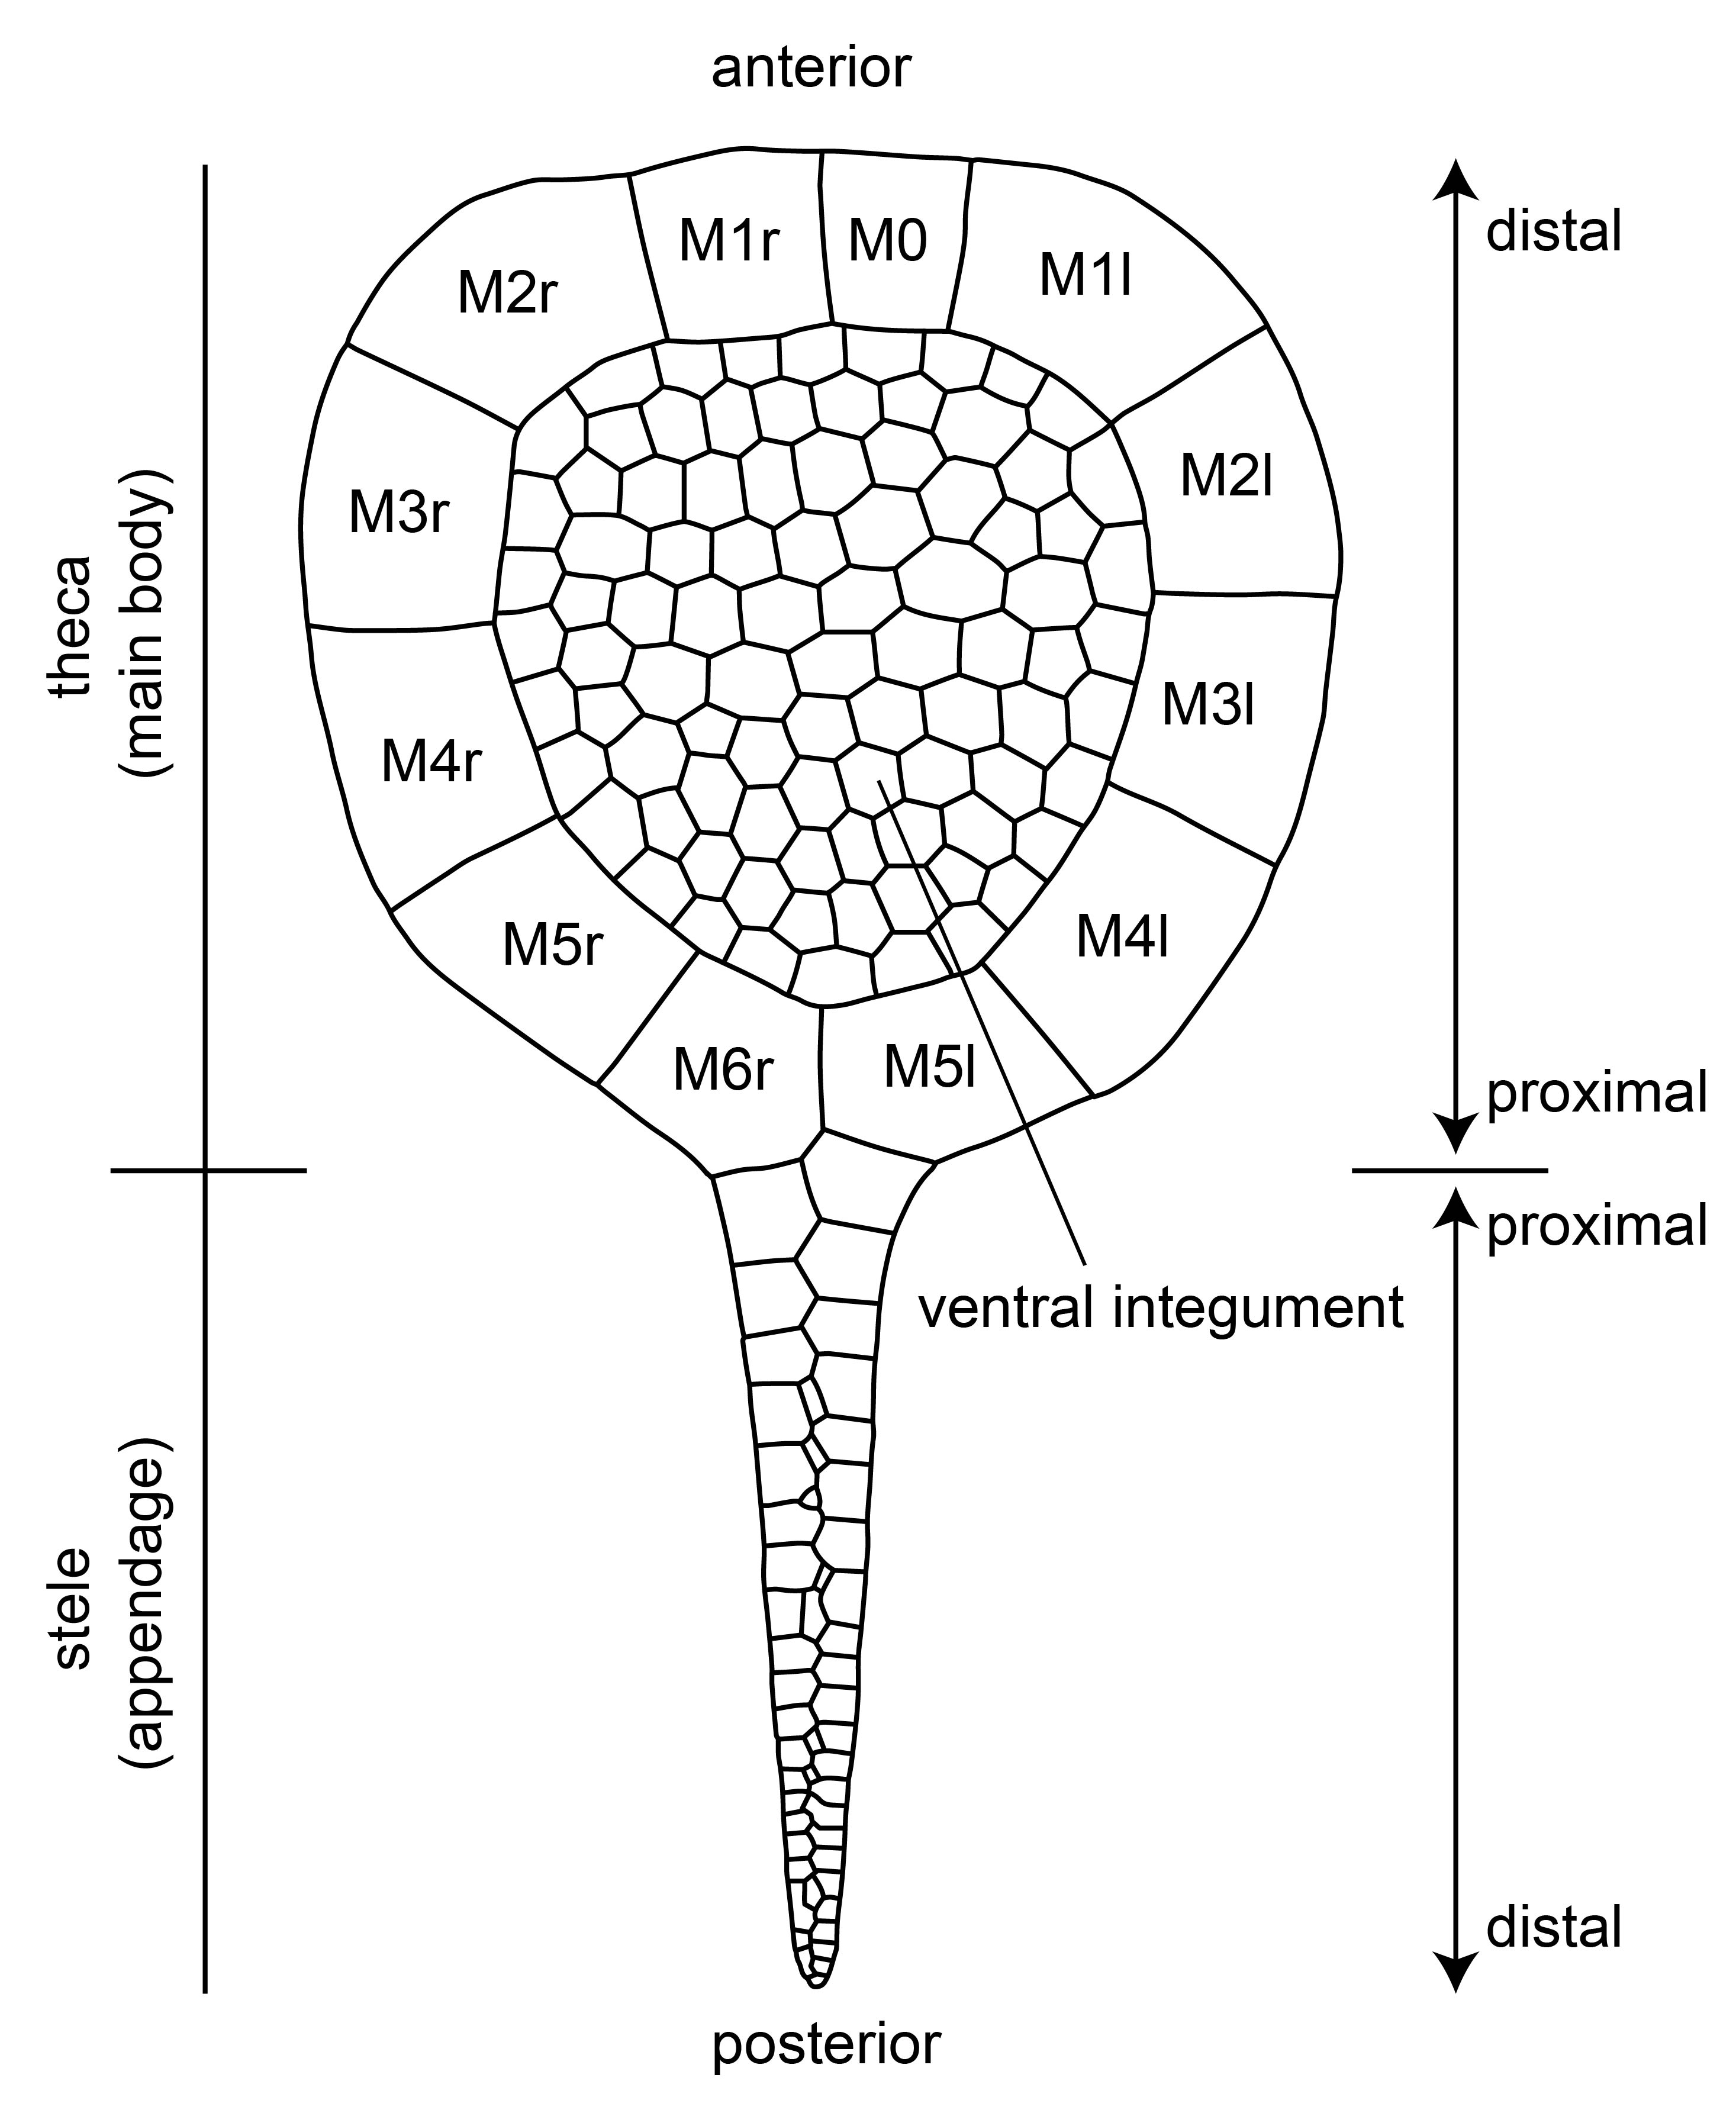
\includegraphics[width=\textwidth]{figures/Cinctan_diagram-01.jpg}
  \caption{Generalized diagram of cinctan morphology based on the ventral side of \textit{Trochocystites}. Marginal plates, i.e., comprising the cinctus, are labeled from the anterior to posterior following \cite{Freidrich1993}; “l” and “r” refer to the left and right side of the theca in dorsal view. See \cite{SmithZamora2009} and \cite{Rahman2016} for additional views of fossils and their anatomical reconstructions.}
\end{figure*}

\subsection{Character Data}
We use the character data initially published by \citep{SmithZamora2009} and subsequently augmented by \citep{ZamoraRahmanSmith2013}.  The analyzed matrix includes 22 cinctan species plus one outgroup taxon (\textit{Ctenocystis}, represented by \textit{Ctenocystis utahensis}). An additional four cinctan species are excluded due to inadequate material for coding.  We refer the readers to the papers cited above for additional information concerning the character data.
\begin{figure*}
  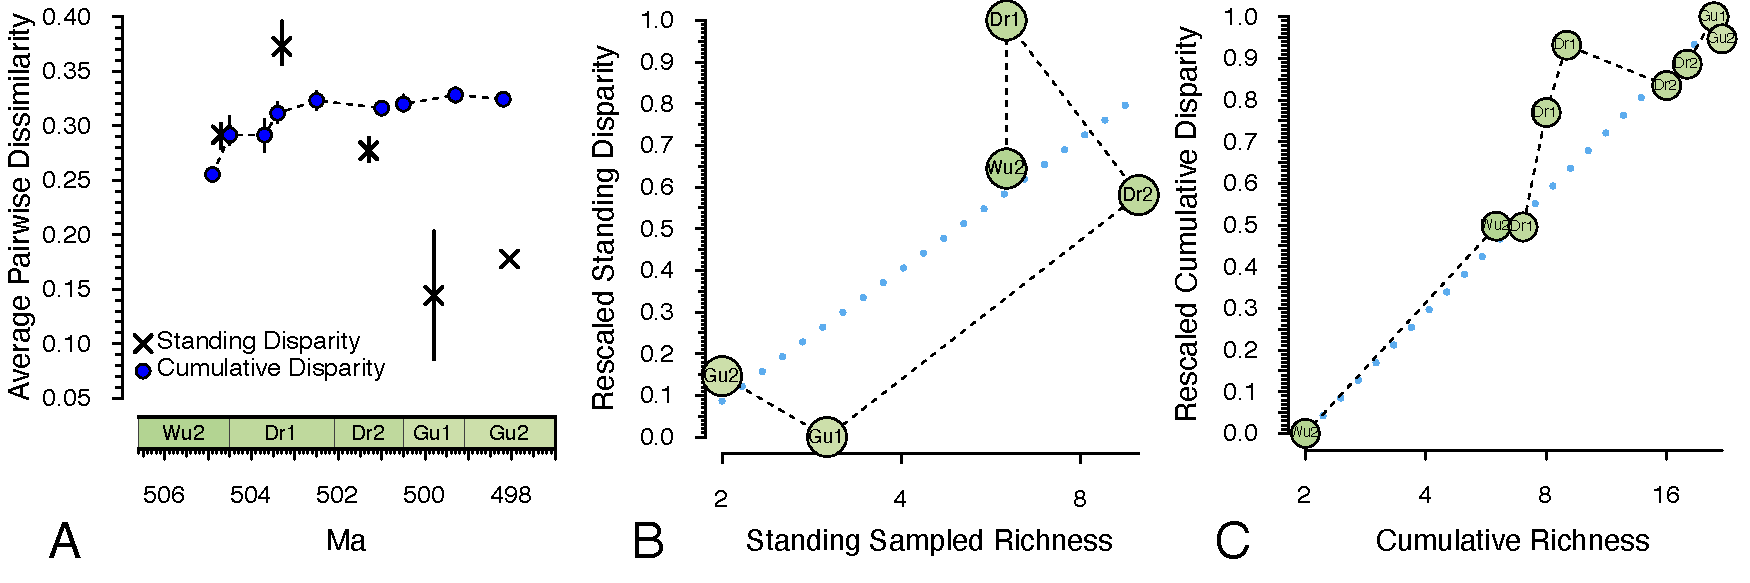
\includegraphics[width=\textwidth]{figures/Cinctan_Disparity_3Ways_Horizontal2.pdf}

  \caption{Disparity patterns for cinctans.  A. Disparity over time based on average pairwise dissimilarities among taxa (see \cite{Foote1992}).  Vertical bars represent 90-percentile error bars from bootstrapping pairwise comparisons \citep{Foote1993}.  X gives "traditional" standing disparity, which reflects only species extant during a stage-slice (see, e.g., \citep{Hughes2013}).  Note also that a minimum of 2 species must be present. Circles give the cumulative disparity among all members of the clade sampled in rocks that age or older, regardless of whether they are still extant and thus depicts the total range of anatomical types derived within the clade \citep{Wagner2015}.  B) Rescaled standing disparity vs. log-taxonomic richness. The dashed line here and in C) give the expected change given continuous rates of morphological innovation.  Because cinctans begin with relatively high richness and then decline over time, the curve begins near the middle of the plot rather than near the bottom as is typical \citep{Jablonski2020}. Note that initial disparity increases markedly despite no increase in standing richness. C) Rescaled cumulative disparity given cumulative richness.  The scale here is finer as it reflects disparity evolved through points in time rather than extant during stage slices. The rapid rise in disparity from the Wuchiapingian to the early Drumian in A) and B) now reflects a the appearance of very anatomically disparate species in the early Drumian while earlier species introduce disparity comparable to that introduced by late Drumian and later species.}
\end{figure*}

Both disparity analyses of these data conducted and arguments pertinent to early echinoderm evolution in the literature (e.g., \citealp{SmithEtAl2013}) suggests that cinctans might exhibit "Early Burst"-type dynamics (Figure 2A), in which a broader range of anatomies appears early in clade history than expected if rates of change were reasonably consistent over time.  Standing disparity vs. log-standing richness patterns deviate strongly from expectations given constant rates of change (\citealp{Jablonski2020}; see also \citealp{Wright2017}), but this reflects in part the clade decreasing in richness through its later history.  The same relationship with cumulative disparity (i.e., disparity among all species known by some date) shows a weaker trend towards higher disparity than expected during the first half of clade evolution (Fig. 1C).  This in turn suggests that rates of change might have been higher early in clade history \citep{Foote1996b}. 




\begin{table}[]
\caption{Chronostratigraphic information for analyzed taxa based on occurrences in the Paleobiology Database.  FA and LA denote first and last appearance dates, with LB and UB giving the oldest and youngest possible FA and LA given the finest chronostratigraphic resolution possible (e.g., a trilobite zone or local chronostratigraphic unit). “N\textsubscript{S}” gives number of sites (= collections or localities) that a species occupies.  “N\textsubscript{R}” gives number of rock units (formations or members) that a species occupies. Dates for \textit{Ctenocystis} represent the entire genus; however, the coded species (\textit{C. utahensis}) is also the oldest known \textit{Ctenocystis}.} 
% Please add the following required packages to your document preamble:
% \usepackage[table,xcdraw]{xcolor}
% If you use beamer only pass "xcolor=table" option, i.e. \documentclass[xcolor=table]{beamer}
\begin{tabular}{l|llllll}
\rowcolor[HTML]{C0C0C0} 
Taxon                                                 & FA\textsubscript{LB}  & FA\textsubscript{UB}  & LA\textsubscript{LB}  & LA\textsubscript{UB}  & N\textsubscript{S} & N\textsubscript{R} \\ \hline
\textit{Ctenocystis}                 & 506.6 & 506.5 & 501.0 & 500.5 & 4  & 3  \\
\rowcolor[HTML]{C0C0C0} 
\textit{Gyrocystis platessa}         & 504.9 & 504.5 & 501.0 & 499.3 & 13 & 4  \\
\textit{Gyrocystis testudiformis}    & 503.1 & 502.5 & 503.1 & 502.5 & 4  & 1  \\
\rowcolor[HTML]{C0C0C0} 
\textit{Gyrocystis cruzae}           & 503.1 & 501.0 & 503.1 & 501.0 & 1  & 1  \\
\textit{Gyrocystis badulesiensis}    & 503.1 & 501.0 & 503.1 & 501.0 & 2  & 1  \\
\rowcolor[HTML]{C0C0C0} 

\textit{Gyrocystis erecta}           & 503.1 & 501.0 & 501.6 & 501.0 & 2  & 1  \\
\textit{Progyrocystis disjuncta}     & 503.1 & 501.0 & 503.1 & 501.0 & 1  & 1  \\
\rowcolor[HTML]{C0C0C0} 
\textit{Protocinctus mansillaensis}  & 506.6 & 505.4 & 506.6 & 505.4 & 1  & 1  \\
\textit{Elliptocinctus barrandei}    & 501.6 & 501.0 & 501.6 & 499.3 & 6  & 3  \\
\rowcolor[HTML]{C0C0C0} 

\textit{Elliptocinctus vizcainoi}    & 504.5 & 503.4 & 504.5 & 503.4 & 1  & 1  \\
\textit{Sucocystis theronensis}      & 501.6 & 501.0 & 501.6 & 501.0 & 2  & 2  \\
\rowcolor[HTML]{C0C0C0} 
\textit{Sucocystis bretoni}          & 501.0 & 500.5 & 501.0 & 500.5 & 1  & 1  \\
\textit{Lignanicystis barriosensis}  & 501.6 & 501.0 & 501.6 & 501.0 & 3  & 1  \\
\rowcolor[HTML]{C0C0C0} 
\textit{Undatacinctus undata}        & 501.0 & 499.3 & 501.0 & 499.3 & 1  & 1  \\
\textit{Sucocystis acrofera}         & 499.3 & 498.2 & 499.3 & 498.2 & 2  & 1  \\
\rowcolor[HTML]{C0C0C0} 
\textit{Undatacinctus quadricornuta} & 501.0 & 499.3 & 501.0 & 499.3 & 1  & 1  \\
\textit{Undatacinctus melendezi}     & 501.0 & 499.3 & 498.2 & 497.0 & 9  & 2  \\
\rowcolor[HTML]{C0C0C0} 
\textit{Asturicystis jaekeli}        & 504.9 & 504.5 & 504.9 & 504.5 & 1  & 1  \\
\textit{Sotocinctus ubaghsi}         & 505.4 & 504.9 & 505.4 & 504.5 & 2  & 2  \\
\rowcolor[HTML]{C0C0C0} 
\textit{Trochocystites bohemicus}    & 505.2 & 504.5 & 503.0 & 502.2 & 4  & 3  \\
\textit{Trochocystoides parvus}      & 504.5 & 503.7 & 504.5 & 503.7 & 1  & 1  \\
\rowcolor[HTML]{C0C0C0} 
\textit{Ludwigicinctus truncatus}    & 501.6 & 500.5 & 501.6 & 500.5 & 1  & 1  \\
\textit{Graciacystis ambigua}        & 504.9 & 504.5 & 503.7 & 503.1 & 3  & 1 
\end{tabular}
\end{table}


\subsection{Chronostratigraphic Data}
Our chronostratigraphic data come from 221 occurrences of Cambrian  echinoderm species from 143 localities last downloaded from the Paleobiology Database (PBDB) on 2020-01-01 \citep{wagner2020}.

The locality and occurrence data came from 81 references with the seven biggest sources including \citet{Nardin2017}, \citet{Zamora2009}, \citet{Chlupac1998}, \citet{Sprinkle2006}, \citet{Termier1973} and \citet{Sprinkle1973}. We ourselves entered 108 of those occurrences and 72 of those localities, and updated 51 of the remaining localities for the purpose of this study.  After accounting for synonymies and variant spellings, the localities represent 55 different rock units (i.e., formations and formations+members).  The accepted names of the species occurrences reflect 361 taxonomic opinions, 155 of which we entered for the purposes of this study.

The Paleobiology Database returns ages based only on the entered interval, which usually is a stage. Here, nearly every cinctan-bearing locality is assigned to the middle Cambrian and thus receives a possible age of 513-501 Ma. However, PBDB provides information allowing much more exact ages. For example, PBDB collection 67775 is one of four including \textit{Trochocystites bohemicus}. This collection is assigned to the Middle Cambrian, and thus is dated by the PBDB as 513 - 501 Ma. However, this collection represents the Skryje Shale, which is known to span four trilobite zones that restrict the age to 505.2 - 500.7 Ma (based on correlations among trilobite zones by \citealp{Geyer2019} to trilobite zone ages in \citealp{Gradstein2012}). Thus, if we had no further information, then that would be the oldest and youngest possible ages for this collection. However, PBDB collection 67775 also is assigned to the \textit{Eccaparadoxides pusillus} trilobite zone, which further restricts the age to 505.2 - 504.5 Ma. We use a database of Paleozoic rock units and faunal zones compiled by one of us (PJW) as a thesaurus to provide more exact earliest and latest possible ages for each cinctan-bearing collection. In addition to refining dates, the database also effectively updates the chronostratigraphic unit to which a locality is assigned if current ideas about the age of a trilobite zone have changed since the paper(s) providing the original data. The typical locality now can be restricted to a 0.7 million year window. Prominent sources for the information relevant to our study and for interregional correlations of rock units and trilobite zones include \cite{Alvaro2001, Linan2004, Geyer2006, Geyer2000, Alvaro2007, Geyer2019}.  The overall timescale is that of \cite{Gradstein2012}. (Note that the more recent timescale of \citealt{Gradstein2020}, which was published after we conducted these analyses, provides nearly identical dates for the relevant Middle Cambrian trilobite zones and thus should not generate markedly different results.)

We use the refined dates to put lower and upper bounds on the possible first-appearance (FA) dates of the cinctan species (Table 1). For species known from only single intervals or trilobite zones, the lower and upper bounds for both first and last appearances are necessarily identical. This is not the case for species spanning multiple intervals. For example, \textit{Gyrocystis platessa} occurs in rocks as old as the \textit{Badulesia granieri} trilobite zone (~504.9-504.5 Ma given \cite{Geyer2019} and Gradstein et al.’s timescale) and also occurs in rocks as young as the \textit{Solenopleuropsis marginata} trilobite zone (~501.0-499.3 Ma).  Here, the latest first possible appearance is 504.5 Ma. We choose the widest possible uncertainty. For example, \textit{Gyrocystis erecta} occurs in rocks belonging to the \textit{Solenopleuropsis} zone (~503.1-501.0 Ma) but also in rocks dated more specifically to the \textit{Solenopleuropsis thorali} subzone (~501.6-501.0 Ma). Because the former set of occurrences might be as old as 503.1 Ma (given existing information), we set the possible lower and upper bounds on the FA for \textit{G. erecta} at FA\textsubscript{LB}=503.1 and FA\textsubscript{UB}=501.0 Ma.

\section{Methods}
\subsection{Estimating starting values for sampling and diversification rates}
We use the Paleobiology Database occurrences described above to derive initial estimates of origination, extinction and sampling for Cambrian echinoderms.  Although this study focuses on just cinctans, other echinoderms represent a taphonomic control for initial estimates of sampling: rocks from environments permitting other identifiable fossils of other Cambrian echinoderms are those in which there is some probability $>$ 0 that we would be able to sample cinctans if they had lived in those environments \citep{BottjerJablonski1988}; in contrast, fossiliferous localities lacking identifiable echinoderms might represent environments in which echinoderms (cinctan or otherwise) lived, but no longer represent sampling opportunities. Other echinoderms also provide a much larger sample size for initial estimates of origination and extinction rates than do cinctans. Although diversification rates likely varied among and within echinoderm clades as well as over time, paleontological data long have suggested that different major clades are typified by general diversification rates \citep{Sepkoski1981}. The larger sample sizes afforded by all echinoderms reduces the chance that our \textit{initial} estimates will be wildly inaccurate as an artifact of sample size. We use a modified version of the Three-Timer method \citep{Alroy2015} that uses lognormal distributions for sampling rates per stage slice rather than a single value \citep{WagnerMarcot2013}. Note that both we use both the diversification and sampling rates to seed the prior distribution with feasible starting values from which to generate new proposals for diversification and sampling parameters in MCMC generations and not as fixed values. Our rationale for adding this extra step is simply that, like all other search algorithms, MCMC analyses beginning with "realistic" parameters should converge on "correct" parameters faster than those analyses beginning with unrealistic parameters; and as diversification and sampling are among the parameters being varied iteration to the next in each analysis, this should make it easier for the analyses to achieve convergence for all of the parameters. We did estimate two parameters that remain static in MCMC analyses directly from PBDB data. One is the probability of taxon-sampling for the youngest species. This parameter is separate from the general sampling parameter because, unlike this analysis, many analyses include extant taxa that have reflect a fundamentally different sampling regime. The other is the earliest possible divergence date for the clade.  We estimate this using the cal-3 metric \citep{Bapst2013}, with the lower bounds set at p=0.003 (i.e., 1-0.05^4). 


\subsection{Models}
The fossilized birth-death is a hierarchical model, meaning that different model subcomponents explain the evolution of the phylogenetic characters (the morphological evolution model), the distribution of evolutionary rates across the tree (the clock model), and the model that describes the speciation (\textit{\textlambda}), extinction (\textit{\textmu}) and fossil sampling intensity (\textit{\textpsi}) leading to the tree (the tree model). 
Below, we describe a hierarchical approach to model-fitting, in which we fit a model to each subcomponent.
The model subcomponents are then assembled into a total fossilized birth-death process.

For each model subcomponent, we first ran an MCMC in RevBayes to assess how long it takes for the analysis to reach convergence. 
Then, using this value, we ran 20 stepping-stone replicates to calculate a marginal likelihood for the data.
Stepping-stone model fitting samples iteratively in the space between the prior and the posterior.
The aim in doing this is to estimate the probability of the data summed over all possible values for parameters  \citep{Xie2011}. 
This enables the calculation of an unbiased marginal likelihood, in contrast to MCMC, which will be biased towards regions of treespace that contain good solutions. 

The result of each stepping-stone analysis is a marginal likelihood.
Because phylogenetic likelihoods tend to be quite small, they are typically reported as log-transformed values.
This means that for model comparisons, we used the log Bayes Factor \citep{Kass1995}, which is represented by the character \textit{K}, and given via the formula:

\begin{center}
  \[  \textit{K}=ln[BF(M0,M1)]=ln[P(X \textbar M0)] - ln[P(X \textbar M1)],  \]
\end{center}    
    
In the above equation, the Bayes Factor for model comparison between Model 0 and model 1 is equal to the probability of the data (X) multiplied by model 0 minus model 1. The final Bayes Factor is calculated by exponentiating \textit{K}:

\begin{center}
  \[  BF(M0,M1)=\textit{e}^\textit{K} \]
\end{center}

The final Bayes Factor is a single value for which a value greater than one constitutes support for model one and a value less than negative one is support for model zero. 

 Within each model subcomponent, Bayes Factors were used to compare different candidate models. 
The winning candidate model for each subcomponent was then used to estimate the subsequent FBD trees.

\subsubsection{Morphological Evolution Models}
We first fit a morphological character model, as no tree can be estimated without one.
We compared three models for morphological character evolution. 
All three were based on the basic Mk model \citep{Lewis2001}. 
In this model, it is assumed that any character has an equal probability change and reversal between any two states. 
The data matrix was partitioned according to the number of character states, so that size of the transition matrix of the model was correctly specified.
In the first model, we did not allow rate heterogeneity. 
In effect, this means we assume all characters to have the same rate of evolution.
In the second, used Gamma-distributed rate heterogeneity to allow different characters in the matrix to have different evolutionary rates.
\citet{SmithZamora2009} explicitly identify characters related to the ``food groove" anatomy of cinctans. A common concern is that characters directly involved with basic organismal ecology and function such as those involved in feeding might evolve under different rules than do other characters \citep{Foote1994,Foote1996a,Wagner1995,Sanchez-Villagra1998,Ciampaglio2002,HopkinsSmith2015, Wright2017}. Obviously, functional morphology of completely extinct groups such as cinctans resides in the realm of hypothesized rather than observed, even if those hypotheses can be corroborated (e.g., \citealp{RahmanEtAl2020}). This situation is akin to knowing that cinctans achieve high disparity rapidly. In that case, we have evidence for rate heterogeneity over time and/or among branches, and not allowing for this should make it more difficult to infer phylogeny accurately. Here, we have reason to suspect that two sets of characters are evolving at different rates, and not allowing for this also should make it more difficult to infer phylogeny accurately. Therefore, we executed partitioned analysis in which feeding and non-feeding characters both have their own Gamma-distributed rate variation parameter should generate more probable overall hypotheses than analyses in which both partitions share the same Gamma-distributed rate variation parameter. Just as rejecting strict clock models in favor of early-burst or relaxed clock models informs us about more than phylogenetic relationships, rejecting a single partition in favor of ``feeding vs. non-feeding" corroborates Smith and Zamora's original interpretation of the characters as well as refining our phylogenetic inferences. Conversely, failing to find a meaningful difference suggests that either the interpretations are incorrect, or that cinctans are a group in which feeding and non-feeding characters evolve at similar rates. Our ``feeding vs. non-feeding" partitioned analysis doubles the total number of parameters by applying each to both character sets independently.

Our MCMC analyses reached convergence after about 80,000 generations, as checked in the software Tracer \citep{Rambaut2018}. 
Stepping stones should generally be run to approximate convergence per stone.
Therefore, each stepping stone was run for 100,000 generations to account for any late-converging stones.

\begin{figure*}
  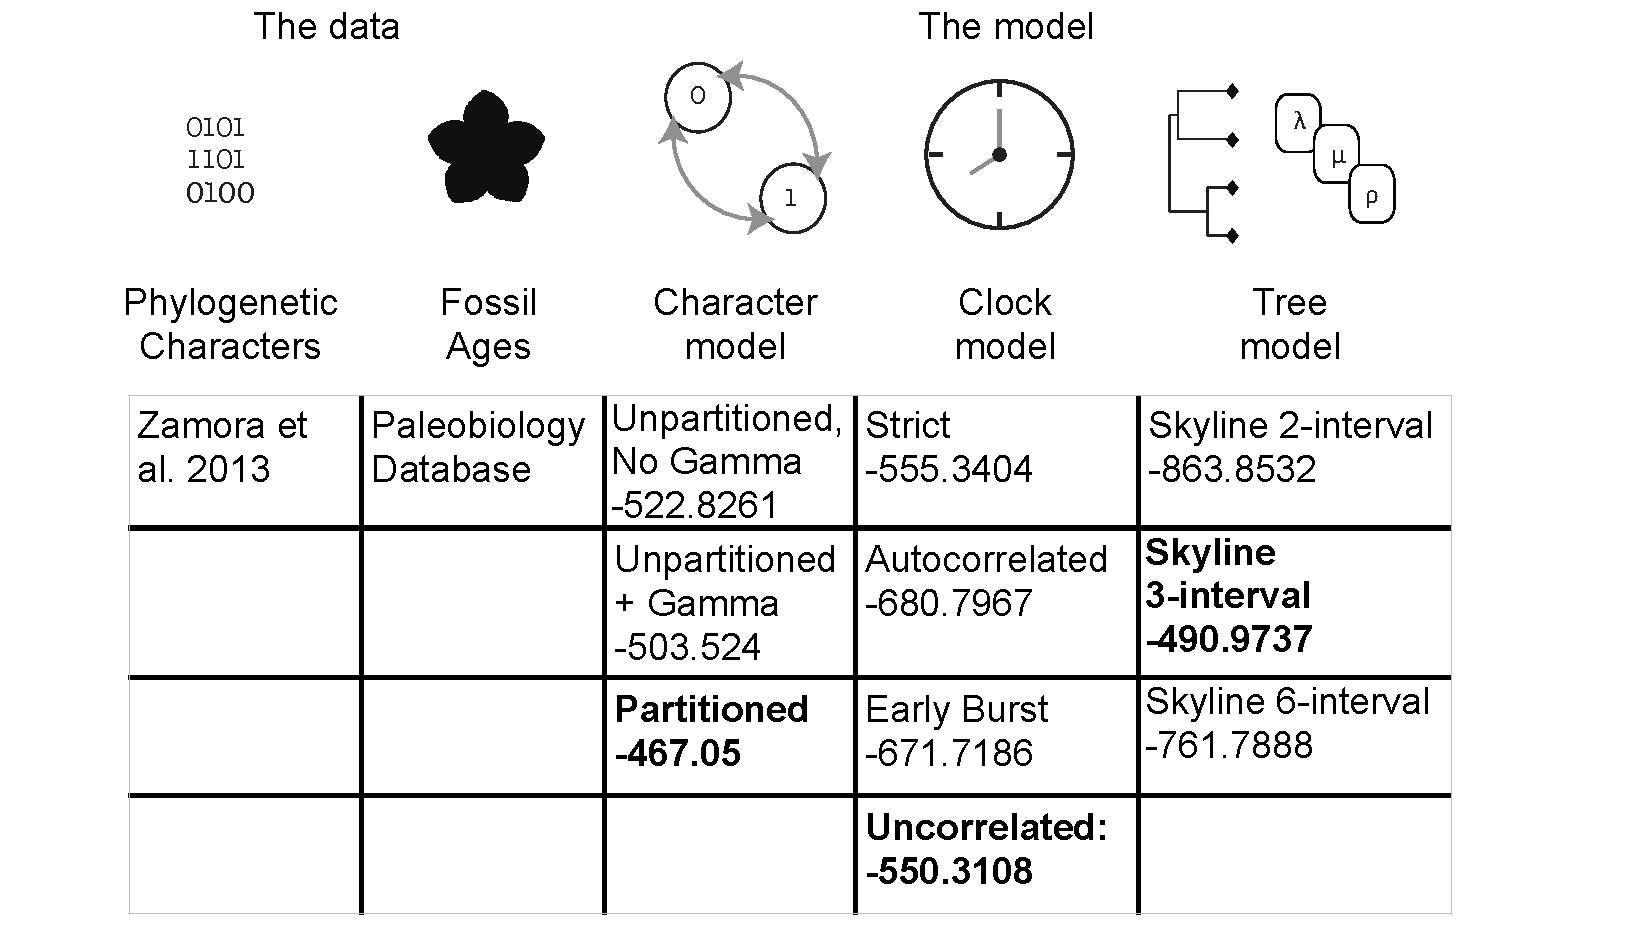
\includegraphics[width=\textwidth]{figures/Fig2.pdf}

  \caption{A table of the competed models for each component of the FBD process, and constituent parameters speciation (\textit{\textlambda}), extinction (\textit{\textmu}) and fossil sampling intensity (\textit{\textpsi}. Underneath each model component are the models competed for that component. The model indicated in bold text is the one that fit the data best, per Bayes Factor model selection.}
\end{figure*}


\subsubsection{Clock Models}

A phylogeny cannot be estimated without a model of character evolution. %Pete to others: Would it be better to state "Phylogenies alone do not have likelihoods given character data; instead, it is the combination of phylogeny (including both general relationships and divergence times) plus character evolution models that have likelihoods given character data."
Hence, the morphology model was fit first.
Next, we fit a clock model.
Although ``clock" might conjure images of a constant rates model, that is only one type of clock (i.e., a ``Strict Clock"): clock models include a range of models that either directly predict or at least constrain plausible rates of change. % Pete to others: I think that this line might help paleo-types: we tend to equate "clock" with "strict clock"
Without a morphology model, no tree can be estimated.
Without an FBD model, age information cannot be included.
Therefore, in order to fit a clock model, we used out best-fit morphology model and a simple, time-homogeneous FBD model to compete different clock models against one another.

The four candidate clock models were as follows.
\begin{itemize}
    \item A strict clock: In this model, the rate of evolution along each branch is assumed to be equal. The rate of evolutionary change is sampled from an exponential distribution. 
    Note that the strict clock model is the most simple clock model, and also (an) equivalent to null models used in paleontological rate studies. 
    It assumes that all branches follow a single, constant rate of morphological evolution. 
    Although simplistic, some studies have found surprising degree of concordance with fossil data fitting a strict morphological clock even when models incorporating rate variation provide a better statistical fit \citep{Drummond2016, Wright2017jp}
    The strict clock model has one advantage in its simplicity: it adds only one parameter to the analyses, whereas relaxed clock models require many additional parameters.
    This clock can be thought of as a null model of evolutionary rate variation.
    \item An uncorrelated lognormal clock: This clock treats each branch as an independent draw from a distribution \citep{Drummond2006, Drummond2007}.  
    In this case, we used a lognormal distribution, which says most evolutionary rates are likely to be low, but with allowances for some branches to have very high rates. 
    It should be noted that because each branch is a separate draw, the rate of an ancestral branch's evolution may be very different than its descendants - either greater or lesser.  In terms of macroevolutionary theory, an uncorrelated clock model is consistent with there being no shifts in intrinsic constraints on rates of change within a clade, but where there is considerable heterogeneity in the effects of ecology on rates of change among different lineages.  
    \item Autocorrelated clock: These clocks assume that the rate of evolution on a descendent branch is drawn from a distribution centered on the rate of evolution of that branch's ancestor \citep{Aris-Brosou2002}.  Here, the rate is heritable, but constantly changing in a manner analogous to a morphometric character under continuous change.  Theoretically, we might expect this if rates are affected by some other variable that is continuously changing (e.g., climate variables or biological variables such as metabolism or size, see further discussion in \cite{bromham1996, gaut1992,thomas2006,bromham2015}).  % Pete to others: does this suggestion make sense? AMW: Yes.
    Thus, this will favor smaller rate shifts than those seen in an uncorrelated clock. 
    The amount of change expected between ancestor and descendant was modeled with a lognormally distribution.
    This assumes most descendants will have a similar evolutionary rate to their ancestors, but allows for some to have a larger disparity.
    \item Early Burst: This clock models treats rates of character change as exponentially decaying over time. 
    This assumes that rates of evolution are fastest near the base of the tree, and decline into the present. 
    As illustrated above, disparity patterns within the clade also suggest this (Fig. 1).
    Prior work has sought the question of detecting radiation in a phylogenetic context \citep{Liow2010}.
    This model builds on this idea while explictly including fossils \citep{Quental2009, Quental2010}. %Davey to others: to my knowledge, this is the first implementation of an Early Burst model specifically implicated in the *inference* of phylogenies (as opposed to post-inference analysis of trait evolution). Is that correct? And if so, should we mention it?
\end{itemize}

Each of these models has a different number of parameters and took a different amount of time to converge. Therefore, for each model, we first ran an exploratory MCMC to see how long convergence takes. Then we used the convergence value to choose the number of iterations per stepping stone.
A table of competed models can be seen in Figure 3.

\subsubsection{Tree Models}

In all of our comparisons of tree models, we used variants of the fossilized birth-death model.
We competed several models, reflecting different scenarios of diversification and sampling in the group.
The simplest model treats these rates as constant over time.  
Of course, innumerable paleobiological studies indicate that origination, extinction and sampling all vary over time within clades.  Shifts in these rates means that the prior probability of a branch spanning a given amount of time is not constant throughout clade history \citep{Wagner2019}. % Pete to others: I figured that some background explaining why this is important might help: sorry to blow my own horn!
Skyline models (e.g., \citealp{Stadler2013b}) treat this as a possibility within FBD analyses by allowing all three rates to vary in different time-intervals. 
We contrasted several skyline models. %Several models competed are termed skyline models. 
These models assume that the parameters of the FBD analysis can vary between discrete time bins. The cinctan fossil record spans three geological stages of the middle Cambrian: the Wulian, Drumian, and Guzhangian. Most of the known species appear in the late Wulian and Drumian, with a marked decrease in the Guzhangian (Table 1).  This suggests temporal variation in origination and/or extinction rates.
Therefore, we allowed all analytical parameters to vary between all three geological stages.
It should be noted that for all skyline models, there is an additional interval of time from the origin to the first interval with its own possible origination, extinction and sampling rates.

\begin{itemize}
\item Time-homogeneous: The first FBD model is a time-homogeneous model in which it is assumed that one rate of speciation, extinction, fossil sampling and sampling at the last occurrence time apply to the whole tree. Note that in Fig. 3, every analysis in the "clock model" column used the time-homogeneous FBD because we need an FBD model in order to incorporate fossils.
\item Two intervals: We tested a model in which the Drumian stage is split into two stages, for a total of two skyline categories (Wuliuan \& Drumian 1, Drumian 2 \& Guzhangian).
\item Three intervals: We tested a model in which each stage is given its own set of FBD parameters, for a total of three skyline categories.
\item Six intervals: In this model, we allowed each stage-slice to have its own rates.
\end{itemize}
Although most prior FBD analyses treat origination and extinction as independent variables, paleobiological studies show that the two are closely correlated (e.g., \citealp{Marshall2017}). 
Over long periods of time, the relationship is nearly linear within large clades (e.g., Figure 4A, illustrating prominent Cambrian to Silurian clades). 
There is more variation with clades over short periods of time such as the stage-slices that we use for these analyses (Figures 4B-C). 
However, there is still a distinct lognormal relationship between origination and extinction. Moreover, the lognormal relationship for only Cambrian stage-slices or for echinoderms by stage-slice fits the same overall lognormal relationship well.  
Thus, our MCMC searches vary origination as an independent variable, and vary turnover (extinction/origination) as a variable dependent on origination. For the time-homogeneous model, this reflects the linear relationship shown in Figure 4A (where turnover varies from 0.90 to 1.05 times origination).
For skyline models, turnover follows the lognormal relationships illustrated in Figures 4B-C.
\begin{figure*}
  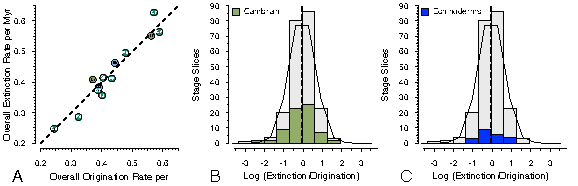
\includegraphics[width=\textwidth]{figures/Turnover_PaleoStyle.pdf}

  \caption{Relationships between origination and extinction rates given birth-death-sampling analyses given Cambrian to Silurian data from the Paleobiology Database.  A. Most-likely origination and extinction rates for species over entire histories of prominent higher taxa: trilobites (Tr), linguliform brachiopods (Li), conodonts (Co), poriferans (Po), tabulate corals (Ta), rugosan corals (Ru), rhynchonellate brachiopods (Rh), strophomenate brachiopods (St), cephalopods (Ce), crinoids (Cr), gastropods (Ga) and bivalves (Bi). Olive green denotes members of Sepkoski's Cambrian fauna \citep{Sepkoski1981} dark green denotes members of Sepkoski's Paleozoic fauna, and light blue denotes members of Sepkoski's Modern fauna. B \& C. Distribution of logged turnover rates for individual clades (including but not restricted to the 12 groups in Fig. 3A) and individual stage-slices (see \cite{Bergstrom2009}, \cite{Cramer2011} and \cite{Rasmussen2019} for stage-slice definitions.)  The best-fit lognormal distribution also is illustrated.  B) Turnover rates for Cambrian time-slices separated.  C) Turnover rates within echinoderm classes separated. }
\end{figure*}

Finally, for all competed models, the best-fit character change model and clock model were used as the other model subcomponents.

\section{Results}

\subsection{Model fitting}

Model selection supported the choice of substitution model with feeding and non-feeding characters (posterior probability: -467.053) modeled separately (log Bayes Factor: 2.938).
It should be noted that Bayes factor support values may appear small, but still reflect significance per the scale in Kass and Raftery (\citeyear{Kass1995}).
An uncorrelated lognormal clock (posterior probability: -550.311) was favored over an autocorrelated clock (posterior probability: -680.797), a strict clock (posterior probability: -555.3404), or "early burst" dynamics (posterior probability: -671.719) with a log Bayes Factor of 4.768 (substantial evidence).
Finally, the three-time interval model (posterior probability: -490.9737) was supported over the two-interval (-863.8532) and six-interval (-761.7888) models (Bayes factor 5.809, substantial evidence). 
A schematic of the model competed with the best-fit models highlighted can be seen on Fig. 3.
Parameters of the best-fit FBD model can be seen on Table 2.

\subsection{Cinctan phylogeny}

The phylogeny estimated can be seen in Fig. 5.
As expected, \textit{Ctenocystis} is sister to the cinctans. 
\textit{Protocinctus}, which has been recovered in some recent studies as nested deep within the cinctan clade \citep{SmithZamora2009}, is recovered here as sister to the rest of the clade. 
The genus \textit{Gyrocystis} is monophyletic, with several species placed as sampled ancestors within the clade. 
 \textit{Progyrocystis} appears in a clade with \textit{Asturicystis} and \textit{Graciacystis}. 
This clade is sister to the \textit{Gyrocystis}, albeit with low posterior support. 
\textit{Trochocystoides} and \textit{Trochocystites} are nested deeper in the tree than in prior analyses, and are more closely related to species within the Sucocystidae.
Similar to prior studies \citep{SmithZamora2009,ZamoraRahmanSmith2013}, we also recover a clade comprising the genera \textit{Sucocystis}, \textit{Lignanicystis} and \textit{Ellipticintus}, though in this analysis \textit{Sucocystic acrofora} groups with the \textit{Undatacinctus}-\textit{Ludwigicinctus} subclade of Sucocystidae.
The HPD on the age of the origin of Succocystidae is between 505.365 and 507.724 Ma.

\begin{figure*}
  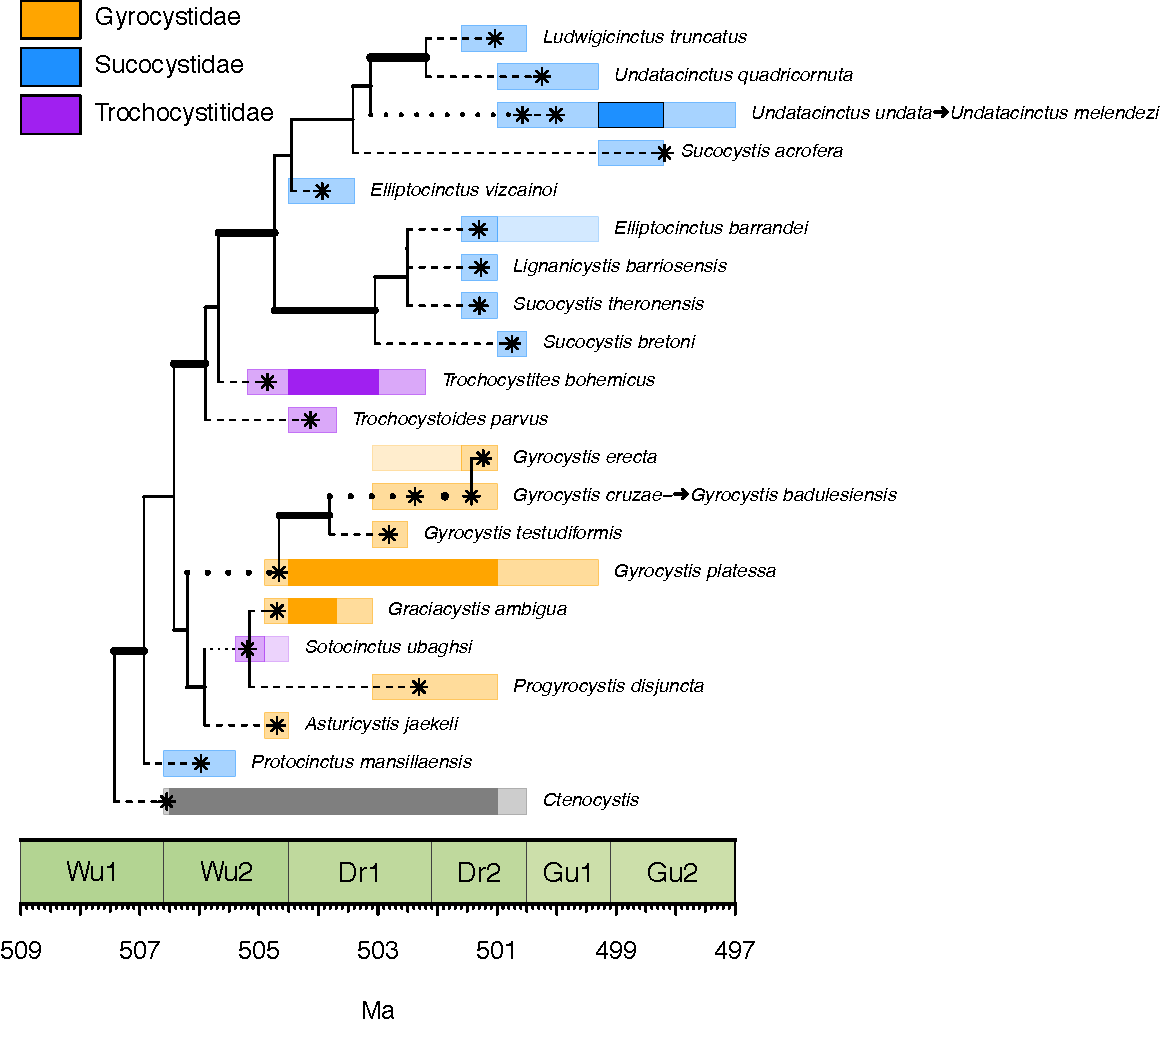
\includegraphics[width=\textwidth]{figures/Pretty Cinctans Families.pdf}

  \caption{A dated phylogeny of the Cinctans. Branch widths of nodes are proportional to the posterior probability of the branch, with wider branches reflecting higher posterior probability. Branch durations preceding sampled species are dashed lines; dashed nodes denote cases where we reconstruct a sampled species as ancestral to the others.  We reconstruct instances where the implied ancestor was still extant when the daughter lineage appears as evidence for budding cladogenesis (see, e.g., \citealp{Eldredge1971}). Asterisks denote most probable ages of first appearances.  For taxon ranges, solid colors reflect ages for which species have definitely older and definitely younger finds; transparent bars represent range of possible first and last appearances.  Extra pale bars represent cases where some of the candidates for oldest/youngest occurrence might be that age. For example,  some occurrences of \textit{Gyrocystis erecta} might be 503.1-501.0 Ma whereas others might be 501.6-501.0 Ma.  }
\end{figure*}

\begin{figure*}
  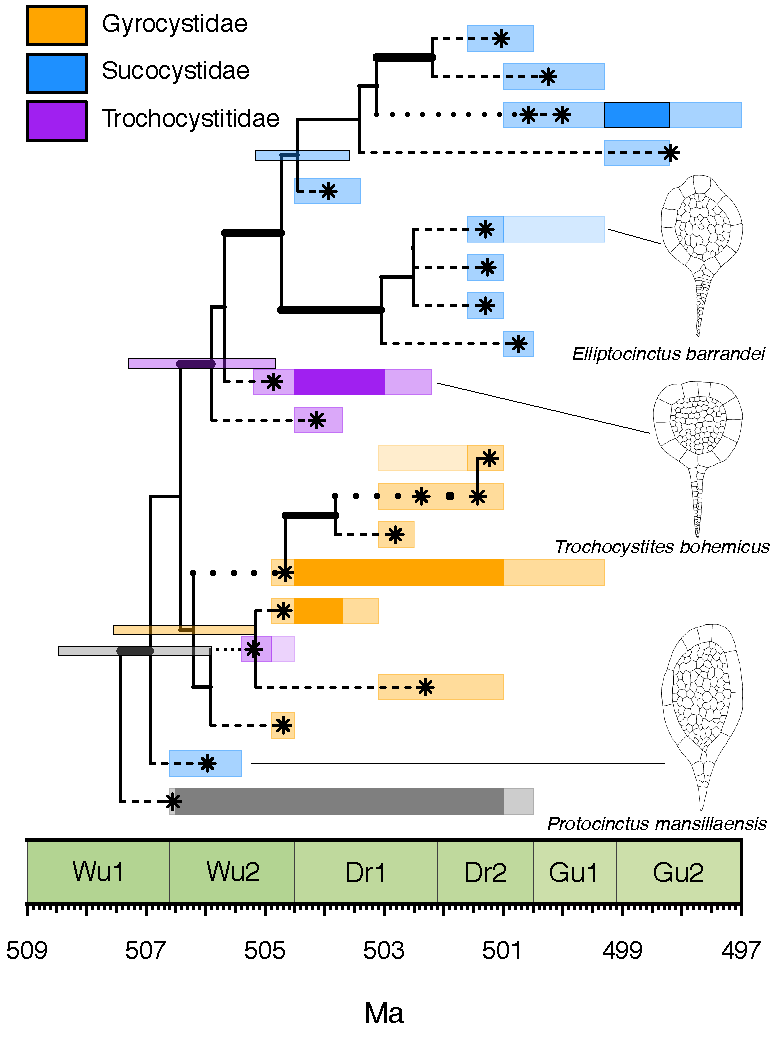
\includegraphics[width=\textwidth]{figures/Pretty Cinctan Divergence Uncertainty_DFW_edits.pdf} 
  
  \caption{The same phylogeny but with credible intervals given for a few major divergences, include: 1) cinctans from ctenocystoids (gray); 2)  gyrocystids from other cinctans (orange);  2)  trochocystitids and sucocystids from other cinctans (purple);  4) sucocystids from trochocystitids.  (Because this tree reconstructs all prior familial definitions as polyphyletic, the clades corresponding to these divergences represent plausible groupings for future revisions to cinctan higher taxa.)}
\end{figure*}

\begin{table}[]
\caption{Diversification parameters of the FBD model. Rates presented as the median of the 95\% HPD of the Bayesian posterior sample for the best-fit model, the model in which each geological stage has its own speciation (\textit{\textlambda}), extinction (\textit{\textmu}) and fossil sampling intensity (\textit{\textpsi}) in parameters. Turnover = \textit{\textmu}/\textit{\textlambda}; Diversification=\textit{\textlambda}-\textit\textmu.
A table with 95\% HPDs for each value can be seen in Table. S1. }
\begin{tabular}{l|lllll}
%Stage      & \begin{tabular}[c]{@{}l@{}l@{}l@{}}Fossil \\ Sampling \end{tabular} & Diversification & Speciation & Extinction & Turnover \\ \hline
Stage      & \textit{\textpsi} & Diversification & \textit{\textlambda} & \textit{\textmu} & Turnover \\ \hline
Guzhangian & 0.188                                                              & -0.193  & 0.493 &  0.687 &       2.148    \\
Drumian    & 0.260                                                            & 0.317    & 1.28 &  0.964 &      0.714  \\
Wuliuan    & 0.224                                                             & -2.657  & 0.916 &   3.574 &      4.936  
\end{tabular}
\end{table}


\section{Discussion}

\subsection{Model-fitting for complex hierarchical models}

When the fossilized birth-death model was first implemented for divergence time estimation, one of the noted benefits was avoiding incoherent fossil calibration points on nodes \citep{Heath2014}.
``Incoherent'' here has multiple meanings: first, that fossils are not data under node calibration methods.
In a node calibration framework, fossils constrain the possible ages a split can have.
The fossil ages ranges are not data under this framework \citep{Gavryushkina2017}.%needs references added
The researcher parameterizes what they believe to be the waiting time between the divergence and this fossil subtending it. 
This waiting time is capturing two different quantities - the uncertainty around the age of the fossil and how long since the divergence the fossil took to arise.
In practice, choice of prior is often subjective, and not based on any one criterion or method, though methods for doing this do exist \citep{Nowak2013}.

The second way in which this practice can result in incoherence is through the collision of priors on different nodes.
Depending on the shape of the prior chosen,  the upper age bound of an ancestor split may conflict with the lower age bound of its descendant splits. 
For example, if a researcher has little intuition for when a fossil arose in relation to the split that it subtends, they may place a uniform distribution specifying the longest and shortest waiting time between the split and the fossil subtending it may be.
Imagine this split and fossil are the descendants of an earlier node, which also has a fossil associated with it. 
Perhaps the researcher has an intuition that this older fossil is likely close to its ancestor node. 
And so the researcher places a lognormal prior on the fossil waiting time, saying the fossil is likely close to the node, but allowing for it to possibly be much older. 
If incorrectly parameterized, the upper bound of the lognormal could overlap the lower bound of the uniform, implying in those cases that the descendant split could occur before the ancestor split.

This is obviously undesirable.
The fossilized birth-death model does not use node calibrations, instead parameterizing the uncertainty of the age associated with each tip.
This is done by placing a uniform prior on each fossil tip that begins with the first occurrence of the fossil and ends with the last occurrence. 
For some taxa, this will mean a fairly wide uncertainty per tip.
For example, in the terrestrial realm, fossil insect occurrences are often dated based on the type of amber they were found in \citep{lapolla2013}. Some ambers can be precisely dated, as the trees that generate the amber has a narrow range.
For others, the range of dates might be quite broad as the amber type could be made from multiple trees, or in tree types with long geological persistences \citep{poinar2000}. In fossils that have been individually dated, this uncertainty may correspond to the uncertainty on the radiometric dating. Similarly, fossil age uncertainty is ubiquitous in the marine fossil record, even for well-sampled fossil taxa. For example, few marine fossils are sandwiched between rock units available for fine-scale radiometric dating. Instead, these layers must be correlated to other units using chronostratigraphic methods, which always involve an envelope of uncertainty. Sometimes, the oldest fossil belong to a particular species may occur just above an unconformity (e.g., a sequence boundary), or stratigraphic correlations of fossil-bearing formations may otherwise be highly uncertain and contentious. Moreover, some fossils, particularly those from historical collections, may have been collected from a locality with low-precision stratigraphic data (i.e., ``Silurian"), with no further information available to narrow its stratigraphic or temporal precision. 
Regardless of the manner in which the uncertainty is derived, the meaning is clear and singular: the uncertainty on a fossil tip represents the minimum and maximum plausible age of the fossil.
This is a far clearer quantity to describe than uncertainty in the age of a fossil, plus the waiting time between the fossil and the speciation that generated it. Critically, it is important to account for fossil age uncertainty in FBD studies, as not doing so can lead to inaccurate inference of tree topologies, divergences times, or both \citep{BaridoSottani2019a,BaridoSottaniEtAl2020}

However, the fossilized birth-death model still contains parameters for which it may be difficult to choose reasonable values.
It is generally known that a small proportion of life that has ever existed has fossilized. 
But what should the fossilization rate in any particular clade be?
Should it change over time? 
Model selection has long been considered an important part of phylogenetic inference \citep{Zwickl2004, allman08b, Baele2013a}.
But in the absence of easy to use selection software (such as the seminal software for molecular model testing, modelTest; \cite{posada1998}), this practice has not been as widely used in other areas systematic research, particularly for divergence time estimation \citep{Duchene2015}.
Here, we have used heirarchical model selection to fit a model for each of the FBD's component submodels.
For each subcomponent, we competed plausible models.
The winning models were combined into a final analysis.
Using stepping-stone model estimation, we were able to calculate precise model likelihoods and use them to compare models using the log Bayes Factor.

While this methodology is computationally intensive, it was also tractable. 
Because no time tree can be inferred without the model to infer a tree first, we first chose our model of morphological evolution.
This is also the least computationally-intense part of the estimation, and can be completed in a few hours.
Using this model, we then chose a clock model, testing four different models (see the next section for a discussion of these models).
Finally, using our morphological evolution and clock models, we competed several versions of the FBD model, including three skyline models.
Scoring a precise marginal likelihood for the total tripartite model is the most computationally intensive part of the work. 
By saving this for last, and first fitting the less parameter-rich morphological evolution and clock models, this estimation is made far more tractable for an average researcher to conduct on a laptop or desktop computer. 

\subsection{What does the chosen set of models tell us?}

Being able to fit a model doesn't mean that fitting that model tells us anything about biology. 
Ideally, we will use our knowledge of the system to turn that model fit into knowledge. 
As shown on Fig. 3, we competed several different models of morphological evolution, clock rate distribution across the tree, and the tree model. 
Each of these models and parameters has meaning in terms of evolution. 
As the biological or geological interpretation of these phylogenetic models may not be intuitive to geologist readers, we will now examine what we have learned about evolution from this exercise.

The model of morphological evolution is intended to capture how the phylogenetic characters have evolved over time.
It is the chief source of information about the topology.
The models of morphological evolution we used were all based on the Mk model \citep{Lewis2001}. 
In this model, it is assumed that characters can be in any one of \textit{k} known character states, that each character can change instantly along a branch, and that probability of change between any two states is equiprobable.
In our analyses, the model featuring rate variation among characters fits the dataset better than a single rate of evolution across a dataset.
This is somewhat unsurprising, as most work in this group has been conducted under parsimony, a model which assumes each character has its own rate of evolution.
We also investigated partitioning in this dataset.
Prior work has been equivocal about whether ``ecological" traits such as feeding structures evolve at higher rates than do other characters, with nearly equal numbers of studies contradicting the notion \citep{Foote1994,Sanchez-Villagra1998,Ciampaglio2002} and supporting it \citep{Wagner1995,Blomberg2003,HopkinsSmith2015}.
Here, we find support for these characters being partitioned, with their own rate heterogeneity parameters, though neither set of characters showed consistently higher rates of evolution. 

We examined four clock models.
The first was a strict clock. 
These types of clocks are rarely supported in molecular systematics.
Rates of molecular evolution are impacted by generation times,  metabolic rate, and mutation rate.
For a more in-depth review of this concept, see Warnock and Wright (2020) in this issue. %needs references added
How this translates to rates of morphological evolution over time is not well-studied, but all the above factors are also likely impact the evolution of anatomical form. 
In general, little correspondence has been discovered between molecular and morphological rates of evolution \citep{bromham2002}.
Therefore, the lack of support for a strict clock in our data is unsurprising.

The remaining three clock models describe more biologically interesting scenarios.
An autocorrelated clock model implies that a descendant branch will have a rate of evolution that is related to the rate of evolution of its ancestor.
This is an appealing model, as we would expect that life history traits that effect possible rates of change may accumulate variation slowly, and be similar to their ancestors. 
We also examined an early burst model, in which the rate of evolution slows over time.
This, too, is an interesting biological hypothesis that is testable given our data.
However, both models were less well-supported than the uncorrelated lognormal clock,
a model in which large changes in rates of evolution can be seen among ancestor-descendent pairs.
It should be noted that while more flexible in terms of the rate variation allowed between ancestors and descendants, the uncorrelated lognormal is not necessarily the most complex model parametrically. 
The strength of support for the most flexible model suggests that perhaps there is a substantial amount of variation that is not being captured by our current generations of clock models.
There may be a universe of models awaiting description that could be tapped into to fill this need.
It is worth noting that in order to compute a clock model, some tree model must be assumed in order to incorporate age information. 
Therefore, the clock model fitting results on Fig. 3 assume a time-homogeneous FBD model. 
It may be worth exploring refitting clock models once the FBD model has been selected.
However, this raises issues of circularity in model fitting procedures that warrant further study.

The final model subcomponent is the tree model.
We were able to easily reject a time-homogeneous FBD model in which one rate of speciation, extinction, and fossil sampling applies across the whole tree.
The entirety of the tree is only a 12 million year span of evolutionary history.
Being able to reject one model over a relatively small amount of time implies that variable-rate models might be appropriate for a great many systems.
Cinctans appeared in a three-stage slice of the Miaolingian Epoch. 
One competed model looked at having the Wuliuan, Drumian, and Guzhangian stages have different sets of FBD parameters. 
Another was  a two-stage model in which time was split down the middle in the Drumian.
And a third, most complex model in which each stage was split into two intervals was also examined. 
It is worth noting that discriminate power between these models was fairly good, and that the most complex model was not simply chosen.
The three-stage model fit best, followed by the six-stage model, and finally the two-stage model. 
This is somewhat comforting: if the most complex model had been chosen for each component model, one would wonder if we were not simply choosing from a candidate set of under parameterized models. 
The Bayes Factor is a reasonably conservative test, and did reject more parameter-rich models in favor of simpler ones.

Together, these models paint a picture of evolution in which trophically-important characters evolve according to different mechanisms than non-trophic characters.
We find evidence for a world in which at times of notable transitions of the Earth (geological stages), we see change in the fundamental processes of diversification and sampling.
And we come to understand that from ancestor to descendant, different life history pressures lead to changes in the rate at which evolutionary change accumulates. 
These first forays into hierarchical model fitting call attention to significant pieces, such as the clock model, where we may be able to examine sources of heterogeneity and improve our models even further.

\subsection{Cinctan phylogeny: implications for systematics and macroevolution}

The origin time of the cinctan-\textit{Ctenocystis} group was 507.52 mya (HPD 505.808 - 508.11 mya), with the ingroup originating at 505.747 mya (HPD 507.27 - 504.699 mya).
As we note in our discussion of the chronostratigraphic data that we use, each tip (i.e., species) has uncertainty associated with its first appearance: we might know that the first occurrence (or possible first occurrences) are in a particular trilobite zone, but that typically restricts the age to a 1-3 million year window.  This might sound trivial if we are thinking about divergences for modern taxa, but here it represents a significant proportion of expected species lifetimes, and thus a potentially large amount of time to accumulate (or not accumulate) character change.
In RevBayes' implementation of the FBD model, tip uncertainty is typically treated as a uniform prior between the first and last appearance on the tip taxon \citep{baridosottani2020}.
The uniform prior says that no age within the bounds is \textit{a priori} more likely than any other.
Nonetheless, we do see significant structure in the distributions for each tip (Fig. S1). 
Some tips, such as \textit{Ctenocystis} and \textit{Elliptocinctus vizcainoi} show strong skew towards the older or younger ages within their uniform tip range.
Others, such as \textit{Asturicystis jaekeli} show less signal, retrieving more-or-less the input uniform prior.
This suggests that FBD analyses may be useful in the future for helping to narrow tip age ranges \citep{Drummond2016, beck2020}.
In clades where tip uncertainty tends to be quite high, this could be an analytical path to higher precision on tip ages.

The topology of the tree is fully-resolved but poorly-supported on many nodes (Figure 5).
This is unsurprising, as bootstrap support values in prior work have also been low \citep{SmithZamora2009, ZamoraEtAl2013}.
The placement of \textit{Protocinctus} is interesting on this phylogeny. 
Although it is the oldest cinctan, \textit{Protocinctus} also possesses some derived character states if we assume that \textit{Ctenocystis} is the appropriate outgroup \citep{Rahman2009a}.  
Accordingly, prior phylogenetic studies place it as a basal member of the Sucocystidae, but evolving after the Sucocystidae diverged from both the Gyrocystidae and Trochocystitidae \citep{SmithZamora2009, ZamoraRahmanSmith2013}. 
The placement of \textit{Protocinctus} as sister to the rest of the cinctans is likely not solely due to the age of the fossil. This fossil is younger than its parent's next several ancestor nodes, meaning it could have been plausibly placed in a more derived position nested within the cinctan clade, but was not in the phylogeny inferred by the best fitting model (see Fig. S2 for alternative positions of \textit{Protocinctus} in sub-optimal models). 
The split between \textit{Protocinctus} and the rest of the cinctans is also one of the most well-supported nodes on this tree.
In trees constructed with the second and third best-fit model, \textit{Protocinctus} is sister to a paraphyloetic grouping of Gyrocystidae and Sucocystidae, and as a sampled ancestor sister to the Sucocystidae (Fig. S2).

In the in-group topology, \textit{Asturicystis}, \textit{Progyrocystis}, and \textit{Graciacystis} form a weakly-supported clade that is sister to the rest of the \textit{Gyrocystis}.
\textit{Trochocystoides} and \textit{Trochocystites} do not form a monophyletic grouping. 
Our phylogeny also reflects a closer relationship between \textit{Undatacinctus} and \textit{Ludwigicintus}. 
Neither \textit{Elliptocinctus} nor \textit{Sucocystis} are monophyletic in this analysis.
Some of these differences may represent differences between the model applied here and in previous work.
We used the Mk model \citep{Lewis2001}, which is more robust to superimposed or homoplasious changes than parsimony \citep{Felsenstein1978, Wright2014}.

But differences may also reflect the inclusion of age information.
For example, \textit{Elliptocinctus} is a genus with two species on this tree, and prior analyses have recovered these as sister taxa.
We did not recover \textit{Elliptocinctus} as monophyletic, with \textit{Elliptocinctus barrandei} descending from a node that is 501.865 million years old (age HPD 500.326 - 503.626 Ma) (Figure 6).
This node is younger than the earliest appearance of \textit{Elliptocinctus vizcainoi}.
In order for these two taxa to be monophyletic, the strength of evidence in the character data would have to be strong enough to either move \textit{Elliptocinctus vizcainoi} into that grouping (which is a canonical position for \textit{Elliptocinctus}), thereby moving the age of the whole group back several million years, or would have to move \textit{Elliptocinctus barrandei} out of it.
Cinctans have a relatively small amount of characters, and our analyses suggests notable homoplasy in the group.
For this reason, the inclusion of other information may be a significant benefit to the accuracy and clarity of phylogenetic and macroevolutionary solutions.
In particular, fossil age information is not confounded by homoplasy.
Fossil age information are treated as data under the FBD model, which has historically not been true of calibration methods, in which fossil age information was used to set constraints on clade ages. 
This means that the age information does not directly constrain the topology.
Topology is determined from the discrete character data.
Fossil age information is used to date the tree and determine which of the topologies are most plausible, given the ages available.
It will be worth further exploration to find out when we expect age information to exert a stronger influence than character information in determining a dated tree.

Interestingly, \textit{Gyrocystis} has a number of sampled ancestors in the genus. In this genus, there are a total of three sampled ancestors, one pair of which (\textit{G. erecta} and \textit{G. badulesiensis}) likely represent budding cladogenesis, i.e., a case of speciation where the ancestral species persists. Its sister group also has one, which may also represent evidence for budding speciation. We emphasize these data show evidence for budding speciation despite the fact that we did not explicitly model stasis nor distinguish between ``punctuational" changes associated with speciation vs. continuous change within lineages (e.g., \citealp{EldredgeGould1972, WagnerMarcot2010}). However, the differences between character changes associated with speciation vs. continuous background change for these data might be small enough to be subsumed by the uncorrelated relaxed clock model we employed, which models rate shifts as occurring between branches but constant across a given branch's duration. Nevertheless, future analyses employing more complex approaches to modeling speciation dynamics in fossil cinctans may outperform the models considered herein.

Evidence for sampled ancestors in the cinctan fossil record might seem surprising given that the echinoderm record is less complete than many other marine invertebrates \citep{FooteSepkoski1999}, although recent FBD studies find strong evidence for their occurrence in the particularly well-sampled record of Paleozoic crinoid echinoderms \citep{Wright2017jp, WrightToom2017}.  However, four of the five cases for cinctans are from the Drumian, for which skyline models imply the highest sampling rate for cinctans. The probability of sampling ancestor-descendant pairs reflect the probability of sampling two species (i.e., [completeness]\textsuperscript{2}, see \citealp{Foote1996c}) is: 
%Davey-- need equation number from Foote1996.I think we'll need to say what psi and mu are if it's not stated somewhere else in the manuscript (I don't think it is?)
%Pete: I put lambda, mu & psi in Table 1. I also added the package that lets us just put Greek letters into the text.
%\[\textit{completeness} = \frac{\psi}{\psi+\mu} \\ %\citeauthor{foote1997estimating}  1997 eq. 1b\]\
%\end{center}
\begin{center}
\[\textit{Pr}\textrm{[sampling} \: \textrm{two} \: \textrm{species]} = (\frac{\psi}{\psi+\mu})\textsuperscript{2} \]
\end{center}
where \textit{{\textpsi}} is the fossilization rate and \textit{{\textmu}} is the extinction rate (see \citealp{foote1997estimating}, equation 1b).
Still, even at the peak during the Drumian, we expect completeness of ~0.21. This in turn predicts that we should find direct ancestor-descendant pairs only 4\% of the time.  However, sampling of ancestors and descendants often should be more probable than global sampling rates imply because sampling rates vary geographically as well as temporally. Because ancestors and descendants usually occur in the same geographic regions and environments, and because ancestors and descendants must at least abut temporally, factors favoring the sampling of any one species often favor the sampling of close relatives, including ancestor(s) \citep{WagnerErwin1995}. 
%Evidence for sampled ancestors in this group is somewhat unsurprising as both turnover (2.138) and fossil sampling (0.188) are relatively high in the time interval in which the taxa occur (Table 2; see \citep{Foote1996c}). 
%Conditions of high turnover should facilitate the evolution of ancestors that don't sit on their own branch, as there is high loss of branches per formation of a branch. % Pete: This confuses me a little.  Are we talking about "grandparent" ancestors that sit on nodes like Sotocinctus ubaghsi?  

%The elevated fossil sampling then makes these ancestors more readily discoverable by human observers. 
%There is still a paucity of empirical literature of when sampled ancestors are expected in natural conditions. 
Cinctans have other paleobiological characteristics that make discovery of sampled ancestors relatively probable: (1) the group occurs over a small window of time, allowing for the assessment of taxonomic completeness, (2) they are marine taxa, allowing for better fossilizaton potential than many groups, such as terrestrial vertebrates, (3) they have mineralized skeletons, and are frequently preserved well enough (often as either molds or recrystallized calcite) to code morphological features, (4) they are numerically abundant fossils, particularly in rocks from the Iberian Chains of Spain and the Montagne Noire of southern France, which enables the collection of multiple specimens and assessment of more complete material, and (5) they are small, making it more tractable to score characters from relatively complete specimens.

One final reason why we might not be surprised to find as many cinctan sampled ancestors as we do stems from the fact that reconstructed ancestors co-occur with reconstructed descendants in some cases (Figs. 4-5).  Budding cladogenesis is consistent with a variety of allopatric speciation models in which biological traits enhancing preservation probabilities (e.g., broad geographic ranges and long durations) also enhance the probability of leaving daughter taxa \citep{WagnerErwin1995}, all else being equal. This becomes particularly relevant because both kinds of occupancy patterns and sampling among contemporaneous species are typically exponential \citep{Liow2013,WagnerMarcot2013,Foote2016}, with common species having individual sampling probabilities much greater than average. Therefore, if high occupancy is linked with the propensity for generating more daughter species, then we expect a fossil record biased in favor of species that had daughter species.  This in turn means that we expect ancestor-descendant pairs to be more common than completeness metrics would predict.  Our results suggest cinctans conform to this general model, and other taxa with similar preservation rates and sampling intensity may also contain sampled ancestors. 







\section{Conclusion}

In this contribution, we have laid forth a framework for fitting complex, hierarchical phylogenetic models. We also draw attention to the relationship between macroevolutionary models on which many paleobiological studies focus and their corresponding phylogenetic models. 
We hope our case study of cinctan echinoderms illustrates how the methodological approaches to phylogenetic paleobiology discussed herein provide useful tools for a diverse range of paleontological interests and pursuits. 
The fossilized birth-death represents a significant leap forward in terms of the integration of fossils in Bayesian phylogenetic analyses. 
Under this model, fossils are data, not mere clade constraints.
However, to leverage this framework involves fitting multiple submodels to a particular dataset.
In doing so, we also inferred a new dated phylogeny for cinctan echinoderms, and provide some insight as to how and why this phylogeny differs from prior work, and highlighted its systematic and macroevolutionary implications for cinctan paleobiology.
We have highlighted several theoretical and empirical concerns, such as how age information impacts topology and how common sampled ancestors are in empirical datasets, which have major implications for discerning models of speciation in the fossil record.
It is our hope that in describing how complex model fitting can be carried out in a tractable way, we will empower more taxonomic empiricists to use the FBD approach we utilize herein with their data.
We believe the interplay between theoretical phylogenetics and deep taxonomic knowledge of empirical paleontologists is critically important for generating models that not only help us better understand the peculiarities of our favorite taxonomic groups, but also help unravel generalities in the history of life.


\section{Acknowledgements}
Supporting scripts can be found in the supplemental code package DOI:10.5281/zenodo.4421405.
This manuscript is one of several associated with the Paleontological Society short course, hosted at the Geological Society Annual Meetings in Phoenix. We thank the Paleontological Society for the support that made the course and manuscript possible.
We thank A. Lin, P. Novack-Gottshall, P. Borkow, P. Hearn and A. Hendy for contributing substantial amounts of the Paleobiology Database information that we use, and S.R. Cole for assistance with obtaining line drawings for fossil cinctans. S. Carlson, S. Zamora, B. Deline, and one anonymous reviewer are thanked for their insightful and constructive reviews.  AMW acknowledges  support from an Institutional Development Award (IDeA) from the National Institute of General Medical Sciences of the National Institutes of Health under grant number P2O GM103424-18. D.F.W acknowledges support from the Gerstner Scholars Fellowship and the Gerstner Family Foundation, the Lerner-Gray Fund for Marine Research, and the Richard Gilder Graduate School, American Museum of Natural History, as well as a Norman Newell Early Career Grant from the Paleontological Society.  This is PBDB Publication  XXXXX.

% Text from Pete below!

%One final reason why we might not be surprised to have as many sampled ancestors as we do stems from the fact that reconstructed ancestors co-occur with reconstructed descendants in some cases (Figs. 4-5).  This pattern (budding cladogenesis) is consistent with a variety of allopatric speciation models in which features encouraging preservation (broad geographic ranges and long durations) also encourage leaving daughter taxa \citep{WagnerErwin1995}. This becomes particularly relevant because both occupancy patterns and sampling patterns among contemporaneous species typically are exponential \citep{Liow2013,WagnerMarcot2013,Foote2016}, with common species having individual sampling probabilities much greater than average. Therefore, if high occupancy encourages generating daughter species, then we expect a fossil record biased in favor of species that had daughter species.  This in turn means that we expect ancestor-descendant pairs to be more common that completeness itself predicts.  Our results suggest that cinctans evolved according to this general model.  

%Note also that trees implying budding cladogenesis typically imply speciational (punctuated) change. However, we did this using the Mk model, which effectively models what \citet{EldredgeGould1972} called "phyletic gradualism" for discrete characters and where \[{\alpha}\textit{t}\]


%Pete: I was just using the textGreek functions to make this readable.  It still can get cut, or moved into our other paper. Davey to Pete: Ah! Sorry. I recompiled the file and noticed this was there and thought it was a mistake on my part.
%gives the expected number of changes over time \textit{t}.  Under speciational change, we expect \textepsilon \textlambda \textit{t} changes over time, where \textlambda is the cladogenesis rate and \textepsilon is the probability of change per speciation event \citep{WagnerMarcot2010}. The only difference in expectations for any one branch is that continuous change always predicts \textalpha\textit{t} changes whereas speciational change predicts \textepsilon(1+\textlambda)\textit{t} changes \textit{if} that branch begins with a cladogenetic event.  This difference might well be small enough to be subsumed by the relaxed clock models that we employ here. However, one key distinction remains: under the speciational model, \textepsilon\textlambda would change as the FBD model alters the speciation rate as well as the speciational change rate.  Accordingly, skyline models would predict shifts in frequencies of change even under constant rate of change. Under the continuous model, there is no such connection and expected change should be completely independent of speciation. Our results suggest that future analyses of the Cincta that employ this approach very well might do even better than the models that we do examine. %\epsilon \lambda t
%Where continuous change and speciational change make truly distinct predictions is for a part of the system that our current methods do not examine: that is, what is the probability of net stasis for species for species such as \textit{Gyrocystis platessa},  \textit{G. ambigua} and \textit{Trochocystites bohemicus} under the Mk model?  This would extend to the probability of net stasis for the several species with uncertain first and last appearances after extending the principles presented by \citet{baridosottani2020}) to determine the probabilities that individual species had particular durations given uncertainty in true first and last appearances. Our results suggest suggest that future analyses of this sort will reject continuous change models in favor of 
%In this way, cinctans may represent a sort of best case for calculating sampled ancestor probabilities.

%Our results demonstrate that for cinctans, and other taxa with similar preservation and sampling intensity, the fossil record may contain many sampled ancestors. In addition to resolving relationships and taxonomic issues, these kinds of phylogenetic analyses also provide a wealth of data for addressing a wide variety of far-reaching issues in macroevolutionary theory, including fundamental questions regarding tempo and mode in evolution and the origin of species.
\bibliography{refs} 
\bibliographystyle{plainnat}

\setcounter{figure}{0}
\makeatletter 
\renewcommand{\thefigure}{S\@arabic\c@figure}
\makeatother

\begin{figure*}
  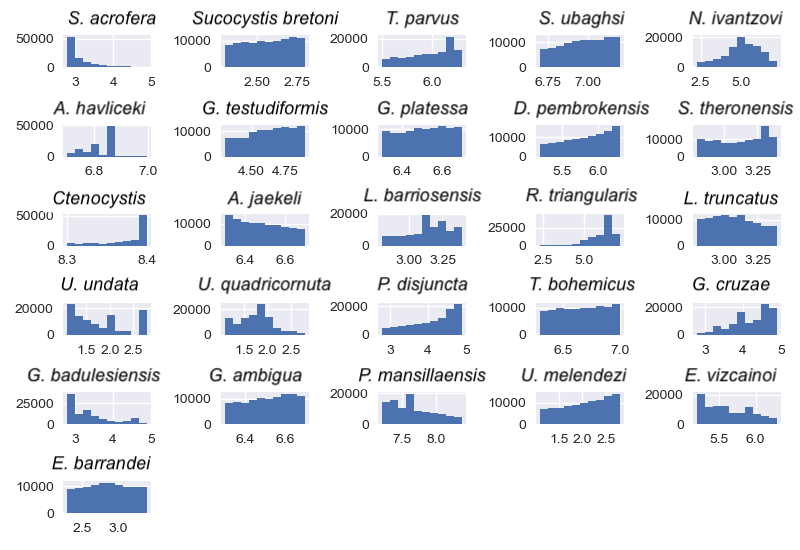
\includegraphics[width=\textwidth]{figures/FigS1.png}
  \caption{Posterior traces for fossil tip ages. These represent the post-burnin distributions of ages recovered for each fossil tip. Uncertainty in tip age was parameterized using a normal distribution between the oldest feasible and youngest feasible ages for each fossil tip. }
\end{figure*}

\clearpage

\begin{sidewaystable}[]
\caption{Diversification parameters of the FBD model. Rates presented as the median of the 95\% HPD of the Bayesian posterior sample for the best-fit model, the model in which each geological stage has its own speciation (\textit{\textlambda}), extinction (\textit{\textmu}) and fossil sampling intensity (\textit{\textpsi}) in parameters. Turnover = \textit{\textmu}/\textit{\textlambda}; Diversification=\textit{\textlambda}-\textit\textmu}. These are the same data as Table One, but with values in square bracket indicating the 95\% HPD of the posterior sample.
\begin{tabular}{l|lllll}
%Stage      & \begin{tabular}[c]{@{}l@{}l@{}l@{}}Fossil \\ Sampling \end{tabular} & Diversification & Speciation & Extinction & Turnover \\ \hline
Stage      & \textit{\textpsi} & Diversification & \textit{\textlambda} & \textit{\textmu} & Turnover \\ \hline
Guzhangian & 0.188 [4.044e-3, 0.589]                                                              & -0.193 [-35.014, 2.859]  & 0.494 [6.145E-5, 2.023] &  0.687 [4.43E-5, 35.473]&       2.148  [.043, 13.044]    \\
Drumian    & 0.260  [3.023e-3, 1.045]                                                           &  0.317 [-37.3075, 2.632]    & 1.28 [2.91E-5, 2.037] &  0.964 [1.68E-5, 37.674] &      0.714 [7.16E-3, 8.783]  \\
Wuliuan    & 0.224   [3.105e-3, 1.089]                                                            & -2.657 [-35.739, 3.181]  & 0.916 [9.57E-5, 2.016] &   3.574 [5.85E-6, 36.524] &      4.936   [6.16E-3, 12.493]
\end{tabular}
\end{sidewaystable}

\makeatother
\begin{figure*}
  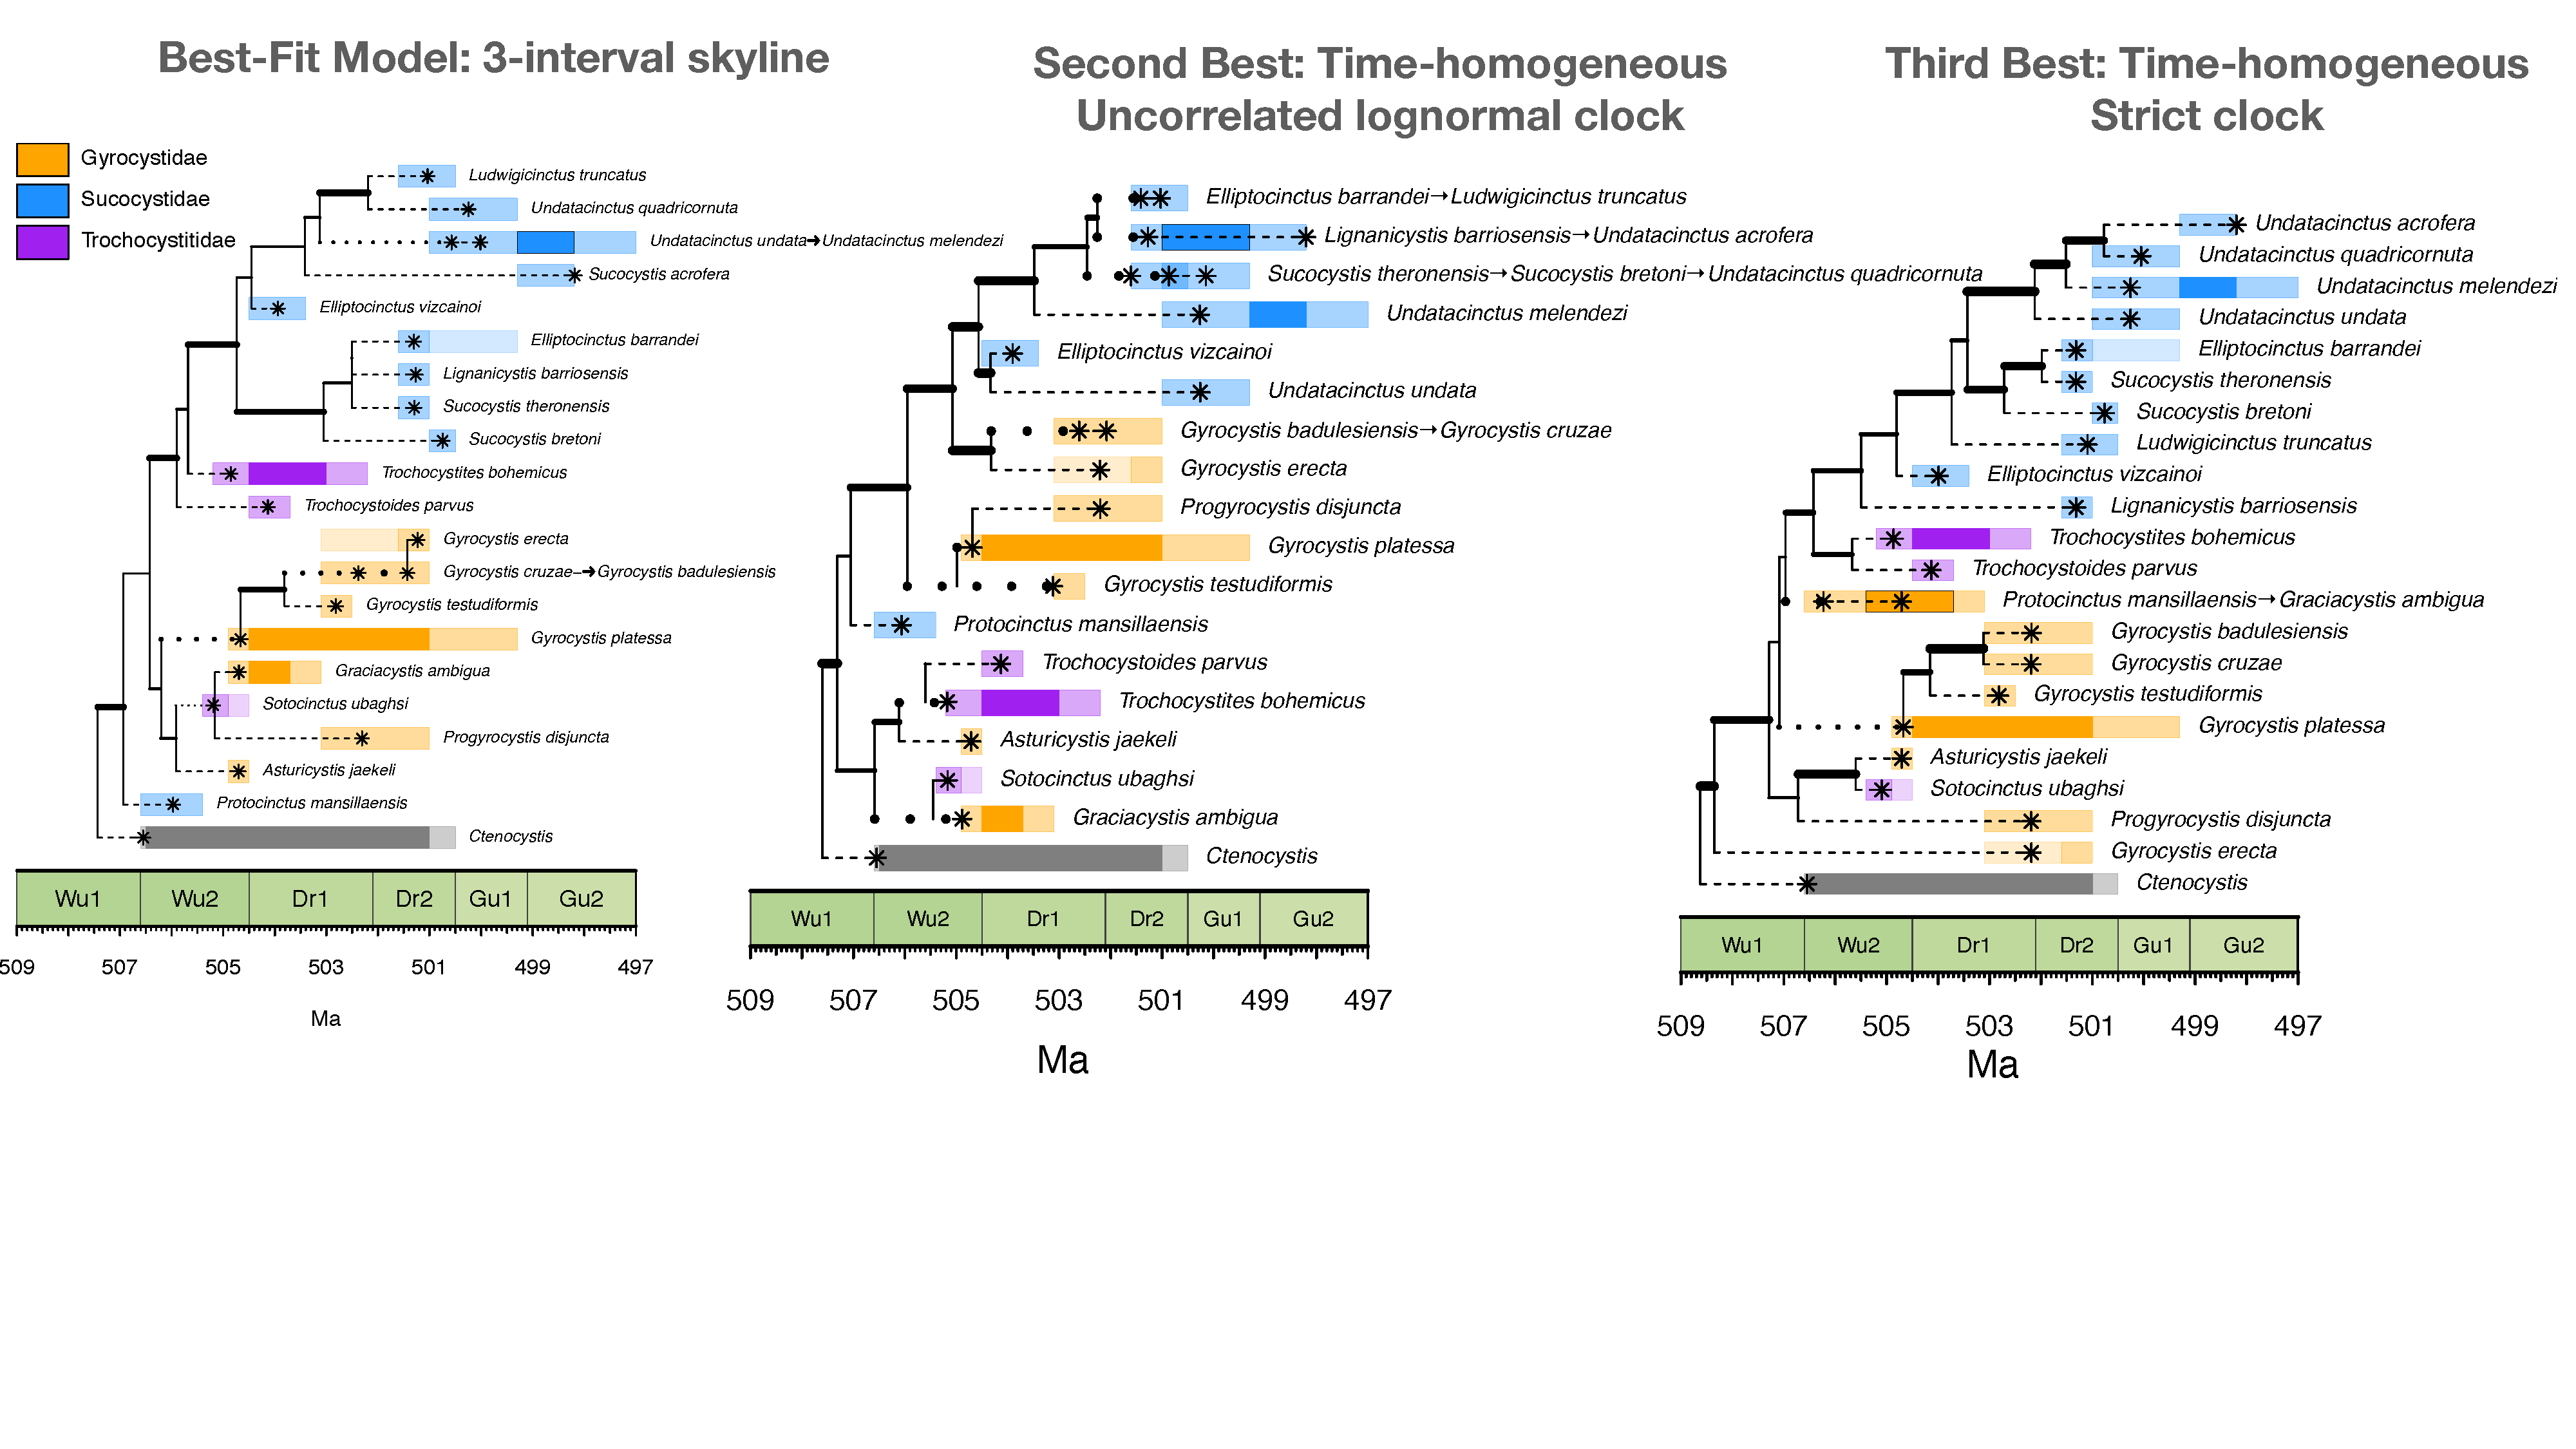
\includegraphics[width=\textwidth]{figures/S2.pdf}
  \caption{Color-coded phylogenetic trees for the top three best models. As can be seen, families are largely similarly grouped between the five hypotheses. The postition of \textit{Protocinctus} varies between the best-fit model and the other two. The number of sampled ancestors also varies among trees. The strict clock tree also contains older divergences internal to the tree. }
\end{figure*}



\end{document}
